\documentclass[10pt]{article}

%%%%%%%% PREÁMBULO %%%%%%%%%%%%
\usepackage[spanish,es-tabla]{babel}
\usepackage[utf8]{inputenc} 
\usepackage{multirow} % para las tablas

\usepackage{tcolorbox}
\tcbuselibrary{listingsutf8}
\usepackage[spanish]{babel}
\usepackage{fancybox}
\usepackage{courier}
\usepackage{ragged2e}
\usepackage[spanish]{babel}
\usepackage[utf8]{inputenc}
\usepackage{amssymb, amsmath, amsbsy} % simbolitos
\usepackage{upgreek} % para poner letras griegas sin cursiva
\usepackage{cancel} % para tachar
\usepackage{mathdots} % para el comando \iddots
\usepackage{mathrsfs} % para formato de letra
\usepackage{stackrel} % para el comando \stackbin
\usepackage{courier}
\usepackage{subfig}
\usepackage{pdflscape}
\title{Plantilla Tesis SEPI ESIME}
\usepackage[spanish]{babel} %Indica que escribiermos en español
\usepackage[utf8]{inputenc} %Indica qué codificación se está usando ISO-8859-1(latin1)  o utf8  
\usepackage{amsmath} % Comandos extras para matemáticas (cajas para ecuaciones, etc)
\usepackage{amssymb} % Simbolos matematicos (por lo tanto)
\usepackage{graphicx} % Incluir imágenes en LaTeX
\usepackage{color} % Para colorear texto
\usepackage{subfigure} % subfiguras
\usepackage{float} %Podemos usar el especificador [H] en las figuras para que se queden donde queramos
\usepackage{capt-of} % Permite usar etiquetas fuera de elementos flotantes (etiquetas de figuras)
\usepackage{sidecap} % Para poner el texto de las imágenes al lado
\sidecaptionvpos{figure}{c} % Para que el texto se alinie al centro vertical
\usepackage{caption} % Para poder quitar numeracion de figuras
\usepackage{commath} % funcionalidades extras para diferenciales, integrales, etc (\od, \dif, etc)
\usepackage{cancel} % para cancelar expresiones (\cancelto{0}{x})
\usepackage[export]{adjustbox}
\usepackage{anysize} % Para personalizar el ancho de  los márgenes
\marginsize{2cm}{2cm}{2cm}{2cm} % Izquierda, derecha, arriba, abajo

\usepackage{appendix} 
\renewcommand{\appendixname}{Apéndices}
\renewcommand{\appendixtocname}{Apéndices}
\renewcommand{\appendixpagename}{Apéndices} 

% Para que las referencias sean hipervínculos a las figuras o ecuaciones y aparezcan en color
\usepackage[colorlinks=true,plainpages=true,citecolor=blue,linkcolor=blue]{hyperref}
%\usepackage{hyperref}
%Para agregar encabezado y pie de página
\usepackage{fancyhdr} 
\pagestyle{fancy}
\fancyhf{}
\fancyhead[L]{\footnotesize ESIME Culhuacan} %encabezado izquierda
\fancyhead[R]{\footnotesize IPN}   % dereecha
\fancyfoot[R]{\footnotesize Grupo 8CV24}  % Pie derecha
\fancyfoot[C]{\thepage}  % centro
\fancyfoot[L]{\footnotesize Ingenier\'ia en Computaci\'on}  %izquierda
\renewcommand{\footrulewidth}{0.4pt}

\usepackage{listings} % Para usar código fuente
\definecolor{dkgreen}{rgb}{0,0.6,0} % Definimos colores para usar en el código
\definecolor{gray}{rgb}{0.5,0.5,0.5} 

% configuración para el lenguaje que queramos utilizar
\lstset{language=Matlab,
    keywords={break,case,catch,continue,else,elseif,end,for,function,
    global,if,otherwise,persistent,return,switch,try,while},
   basicstyle=\ttfamily,
   keywordstyle=\color{blue},
   commentstyle=\color{red},
   stringstyle=\color{dkgreen},
   numbers=left,
   numberstyle=\tiny\color{gray},
   stepnumber=1,
   numbersep=10pt,
   backgroundcolor=\color{white},
   tabsize=4,
   showspaces=false,
   showstringspaces=false}

\newcommand{\sen}{\operatorname{\sen}}	% Definimos el comando \sen para el seno en español


\usepackage{longtable}
%%%%%%%% TERMINA PREÁMBULO %%%%%%%%%%%%

\begin{document}
\nocite{IEEEreferencias:Ref1}
\nocite{IEEEreferencias:Ref2}
\nocite{IEEEreferencias:Ref3}
\nocite{IEEEreferencias:Ref4}
\nocite{IEEEreferencias:Ref5}
\nocite{IEEEreferencias:Ref6}
\nocite{IEEEreferencias:Ref7}
\nocite{IEEEreferencias:Ref8}
\nocite{IEEEreferencias:Ref9}
\nocite{IEEEreferencias:Ref10}
\nocite{IEEEreferencias:Ref11}
\nocite{IEEEreferencias:Ref12}
\nocite{IEEEreferencias:Ref13}
\nocite{IEEEreferencias:Ref14}
\nocite{IEEEreferencias:Ref15}

\begin{center}											            							%%%
\newcommand{\HRule}{\rule{\linewidth}{0.5mm}}	                                               %%%\left
 																								%%%
\begin{minipage}{0.49\textwidth} \begin{flushleft}

\includegraphics[scale = 0.12]{Imagenes/logoesime}
\end{flushleft}\end{minipage}
\begin{minipage}{0.49\textwidth} \begin{flushright}

\includegraphics[scale = 0.25]{Imagenes/IPN}
\end{flushright}\end{minipage}

\vspace*{-1cm}			%%%

\textsc{\huge Instituto Polit\'ecnico Nacional}\\[1cm] 
\textsc{\LARGE Escuela Superior de Ingenier\'ia Mecanica y Electrica}\\[0.5cm] %%%
\textsc{\LARGE Unidad Culhuacan}\\[0.5cm] %%%
\textsc{\LARGE Ingenier\'ia en Computaci\'on }\\[1cm] %%%

\begin{minipage}{0.9\textwidth} 
\begin{center}																					%%%
\textsc{\LARGE REPORTE TÉCNICO}
\end{center}
\end{minipage}\\[0.5cm]
                                                                                    %%%
    																				%%%
 			\vspace*{1cm}															%%%
																					%%%
\HRule \\[0.1cm]																	%%%
\begin{center} \textsc{\Large Desarrollo de una plataforma para la ejecución de pruebas de carga a partir de la definición de un script con JavaScript \\}
\end{center}
\HRule \\[0.1cm]%%%
 										%%%

 																				    %%%



   \vspace{0.8cm}
\begin{center}
{\large Presenta}\\                                                                %%%
Jonathan Eduardo García García\hspace{1cm} jgarciag1404@alumno.ipn.mx
\vspace{1 cm}
\end{center}

\begin{center}
\begin{minipage}{1\textwidth}													    %%%
\begin{flushleft} \large														    %%%
\emph{Asesor del proyecto:}\\
\vspace{0.3cm}
M. en I. TIRSO MARTÍNEZ REYES\\
    \vspace*{1cm}	
                                                                %%%
\end{flushleft}	
%%%
\end{minipage}		                                            %%%
\end{center}

%\begin{minipage}{1\textwidth}													    %%%
%\begin{flushleft} \large														    %%%
%\emph{Directores del proyecto:}\\
%\vspace{0.3cm}
%M. en C. Jose Luis Cano Rosas\\
%Dr. Pedro Guevara L\'opez\

                                                                %%%
 %   \vspace*{1cm}	
                                                                %%%
%\end{flushleft}													%%%
%\end{minipage}		                                            %%%
																%%%
%\begin{flushleft}
 	
%\end{flushleft}
%%%
 		
 		            %%%
\vspace{2cm} 																				
\begin{center}
{\large \today}													%%%
\end{center}												  						

\end{center}
\cleardoublepage


\newpage																		
\tableofcontents 





%%%%%%%%%%%%%%%%%%%%%%%%%%%%%%%%%%%%%%%%%%%%%%%%%%%%%%%%%%%%%%%%%%%%%%%%%%%%%%%%%%%%%%%
%RESUMEN
\newpage
\section{Resumen}
\justify
Está aplicación permite de manera integral la gestión de actividades escolares para los alumnos del  I.P.N., utilizando C\# como lenguaje de programación principal además del framework Xamarin que amplía las funciones de la plataforma de desarrollo .Net con el cual se desarrollaron las principales funciones de la aplicación además usando el lenguaje SQL para el desarrollo de la base de datos  y Amazon Web Services para el almacenamiento está, incluyendo el desarrollo un servicio API para la comunicación entre las peticiones de los usuarios y la base.


\par\vspace{\baselineskip}
\justify
\textbf{Palabras Clave:} Agenda Escolar, Aplicación móvil, Organizador Escolar, Web Scraping, Xamarin.

\par\vspace{\baselineskip}
%%%%%%%%%%%%%%%%%%%%%%%%%%%%%%%%%%%%%%%%%%%%%%%%%%%%%%%%%%%%%%%%%%%%%%%%%%%%%%%%%%%%%%%
%INTRODUCCIÓN 



\section{Introducción}
\justify
Está aplicación permite de manera integral la gestión de actividades escolares para los alumnos del I.P.N. utilizando C# como lenguaje de programación principal además del framework Xamarin que amplía las funciones de la plataforma de desarrollo .Net con el cual se desarrollaron las principales funciones de la aplicación además usando el lenguaje SQL para el desarrollo de la base de datos  y Amazon Web Services para el almacenamiento está, incluyendo el desarrollo un servicio API para la comunicación entre las peticiones de los usuarios y la base.$(\frac{a}{b})^{2}$
%%%%%%%%%%%%%%%%%%%%%%%%%%%%%%%%%%%%%%%%%%%%%%%%%%%%%%%%%%%%%%%%%%%%%%%%%%%%%%%%%%%%%%%
\section{Planteamiento del Problema}
\justify
En la actualidad los alumnos del I.P.N prescinden de un control adecuado de sus actividades  debido a que las mismas se encuentran dispersas en las diferentes plataformas que se usan actualmente, lo cual dificulta una correcta administración de las mismas, así como no tener la facilidad de consultar su horario, calificaciones y perfil estudiantil  de manera sencilla y en un solo lugar provocando una pérdida de tiempo.  Por esta razón se desarrolló esta aplicación para  los alumnos donde pueden unificar todas las actividades escolares además de integrar vistas para la consulta de horario, calificaciones, tareas, recordatorios, enlaces e información del estudiante totalmente personalizada.  

%%%%%%%%%%%%%%%%%%%%%%%%%%%%%%%%%%%%%%%%%%%%%%%%%%%%%%%%%%%%%%%%%%%%%%%%%%%%%%%%%%%%%%%
%OBJETIVOS

\section{Objetivos}
\subsection{Objetivo General}
\justify
Desarrollar una aplicación agenda escolar para  los alumnos del I.P.N. que registre, recuerde, notifique sobre el inicio de cada clase, así como crear tareas, visualizar su horario, calificaciones y progreso escolar para que así el estudiante pueda unificar sus actividades y no estén  dispersas en diferentes plataformas obteniendo un mejor control sobre ellas .

\subsection{Objetivos específicos}

\begin{enumerate}
    \item \textbf{Funcionalidades de Agenda}
    
\begin{enumerate}
\item Desarrollar una vista para la consulta de horario por día y semanal.
\item Desarrollar un flujo que organice y priorice actividades escolares por fecha de entrega.
\item Diseñar una base de datos que permitan almacenar la información de horarios, tareas y recordatorios.
\item Desarrollar y programar una interfaz gráfica intuitiva que presente la información de forma concisa y directa.
\item Cargar el calendario del ciclo escolar en la aplicación para su consulta en cualquier momento.
\item Desarrollar una vista de horario lateral para la pantalla principal que muestre el horario del dia.
\end {enumerate}
\item \textbf{Servicios Web}
\begin{enumerate}
\item Desarrollar un servicio web para administrar y compartir tareas,enlaces y recordatorios
\item Desarrollar una página web para compartir comentarios de cada materia.
\item Integrar un módulo que permite compartir enlaces por materia mediante un servicio web.
\itemDesarrollar un algoritmo que permita consultar las calificaciones del semestre en curso.
\item Desarrollar un foro de comentarios por materia para compartir notas 
\end {enumerate}
\item \textbf{Funcionalidades adicionales}
\begin{enumerate}
\item Desarrollar un foro de comentarios por materia para compartir notas.
\item Desarrollar una vista que permita cambiar la foto de perfil de usuario.

\itemDesarrollar una pantalla con los siguientes datos: nombre, escuela, boleta, carrera, semestre en curso, créditos totales y aproximados, porcentaje de avance.

\item Desarrollar una medida de seguridad biométrica implementando la lectura de huella digital ó reconocimiento facial según las capacidades de cada dispositivo.
\end {enumerate}
\end{enumerate}



\section{Límites y alcances}

\begin{enumerate}
    \item \textbf{Alcances.}

\begin{enumerate}
\item Aplicación desarrollada para  Android y iOS.
\item Extensible a toda la comunidad en modalidad escolarizada.
\end {enumerate}

  \item  \textbf{Límites.}

\begin{enumerate}
\item Diseñado para  alumnos de nivel superior.
\item Autenticación biométrica solo disponible para dispositivos con esta característica integrada.
\end {enumerate}
\end{enumerate}

%Justificacion

\section{Justificación}
\justify
El desarrollo de esta aplicación mejora la organización en las actividades escolares de los alumnos del I.P.N al tenerlas dispersas en diversas plataformas, permite agrupar todas estas actividades en un solo lugar para así tener un control de las mismas, de esta manera se beneficiará a los alumnos de nivel superior del I.P.N, a diferencia de otras aplicaciones existentes en el mercado la aplicación es totalmente personalizada, además de que no es necesario contar con cuentas especiales  que limiten las funcionalidades ya que con ser alumno inscrito en modalidad escolarizada se tiene acceso a todas las funcionalidades de la aplicación. 

%Estado del Arte
\section{Estado del Arte}
\justify
\cite{IEEEreferencias:Ref1} Asistente escolar para los estudiantes de Ingeniería de Software: una aplicación móvil.\\
Aplicación móvil, AcompañaLIS, para los
alumnos de la carrera de Ingeniería de Software de la UADY que les permita el
acceso fácil y oportuno a su información escolar, con el fin de coadyuvar a que
tomen una buena decisión en su carga académica. AcompañaLIS se centra en
proporcionar a los alumnos un medio para facilitar la consulta al Plan de Estudios
de la Licenciatura en Ingeniería de Software, revisando aspectos tales como
requisitos académicos de asignaturas, número de créditos de asignaturas,
duración de la licenciatura, las calificaciones parciales de las asignaturas que
está cursando, y otros más. Aunado a esto, proporciona un canal de
comunicación con el coordinador de la licenciatura, por medio de mensajes al
correo electrónico. 
El  desarrollo de una app y web para el control de la asistencia en las aulas. 
Aplicación web docente para el control de asistencia en las aulas y la publicación de deberes, pensada para centros de Enseñanza Secundaria.
\par\vspace{\baselineskip}
\justify
\cite{IEEEreferencias:Ref2} Aplicación móvil que permite administrar las subscripciones a las distintas clases ofrecidas por la Universidad. Enviar notificaciones de las sesiones de lectura e inicio de clases.


\par\vspace{\baselineskip}
\justify
El \cite{IEEEreferencias:Ref3} smartphone como herramienta de comunicación en el ámbito académico.\\
Conocer cómo perciben los estudiantes el fuso del smartphone con fines académicos y en concreto cualquier aplicación que facilite la comunicación profesor y alumno. 
\par\vspace{\baselineskip}


\par\vspace{\baselineskip}
\justify
\cite{IEEEreferencias:Ref4} Design and Implementation of a Mobile based Timetable Filtering System.\\
Aplicación donde el administrador del sistema define actividades y recordatorios que son enviados a los usuarios del sistema.
\par\vspace{\baselineskip}



Tecnologías de web scraping en un mundo API \cite{IEEEreferencias:Ref10}
\par\vspace{\baselineskip}
\justify
The Comparison of Native Apps Performance on iOS(Swift) and Android with Cross-platform Application-Xamarin \cite{IEEEreferencias:Ref11}
%%%%%%%%%%%%%%%%%%%%%%%%%%%%%%%%%%%%%%%%%%%%%%%%%%%%%%%%%%%%%%%%%%%%%%%%%%%%%%%%%%%%%%%
%Marco Teórico
\section{Marco Teórico}
\subsection{Sistemas de Información}
\justify
Los sistemas de información constituyen uno de los aspectos estratégicos claves para el buen hacer de la empresa. Para ello es necesario que la totalidad de la organización esté concienciada de su utilidad, tanto por parte de la alta dirección, la cual ha de tenerlos en cuenta a la hora de realizar el proceso de planificación estratégica de la empresa, como por parte de los distintos usuarios de la empresa. Ha de existir una política de información y motivación dentro de la empresa. Si esto se lleva a cabo, la empresa logrará superar a sus competidores, podrá aumentar su poder de negociación e incluso podrá evitar la entrada de nuevos competidores logrando la denominada “ventaja competitiva sostenible”. \par\vspace{\baselineskip}

\subsection{Sistemas de Soporte a la Decisión (DSS)}
\justify
Un Sistema de Soporte a la Decisión (DSS) es una herramienta de Inteligencia Empresarial enfocada al análisis de los datos de una organización.
Metodologías, técnicas, mecanismos para recolectar/sintetizar los elementos cuantitativos. \par\vspace{\baselineskip}

\subsection{Base de datos}
\justify
Una base de datos es una colección organizada de información estructurada, o datos, típicamente almacenados electrónicamente en un sistema de computadora. Una base de datos es usualmente controlada por un sistema de gestión de base de datos (DBMS). En conjunto, los datos y el DBMS, junto con las aplicaciones que están asociados con ellos, se conocen como un sistema de base de datos, que a menudo se reducen a solo base de datos.
Los datos dentro de los tipos más comunes de bases de datos en funcionamiento hoy en día se modelan típicamente en filas y columnas en una serie de tablas para que el procesamiento y la consulta de datos sean eficientes. Luego se puede acceder, administrar, modificar, actualizar, controlar y organizar fácilmente los datos. La mayoría de las bases de datos utilizan lenguaje de consulta estructurado (SQL) para escribir y consultar datos. \par\vspace{\baselineskip}

\subsection{Sistema Operativo Android}
\justify
Android es un sistema operativo para móviles diseñado por la compañía estadounidense Google. Basado en el sistema operativo Linux, su objetivo inicial fue fomentar el uso de un sistema de tipo abierto, gratuito, multiplataforma y muy seguro, adaptado a los dispositivos móviles como smartphones y tablets. Desde su creación, el sistema ha realizado una fuerte apuesta para atraer a desarrolladores, por ello cuenta con una variación de Java denominada Dalvik que permite desarrollar aplicaciones que exploten las utilidades de los dispositivos de manera muy sencilla
\par\vspace{\baselineskip}


\subsection{Sistema Operativo IOS}
\justify
iOS es el sistema operativo creado por Apple originalmente para el iPhone que luego fue portado para los iPad y iPod touch. La primera vez que se presentó al público fue en el año 2007 cuando Steve Jobs mostró en la keynote de ese año el nuevo Smartphone que venía siendo desarrollado por la compañía desde hacía unos años. \par\vspace{\baselineskip}


\subsection{Aplicación móvil}
\justify
Una aplicación móvil, también llamada app móvil, es un tipo de aplicación diseñada para ejecutarse en un dispositivo móvil, que puede ser un teléfono inteligente o una tableta. Incluso si las aplicaciones suelen ser pequeñas unidades de software con funciones limitadas, se las arreglan para proporcionar a los usuarios servicios y experiencias de calidad. \par\vspace{\baselineskip}


\subsection{Xamarin}
\justify
.NET es una plataforma de desarrollo compuesta por herramientas, lenguajes de programación y bibliotecas para crear muchos tipos diferentes de aplicaciones.
\justify
Xamarin amplía la plataforma de desarrollador .NET con herramientas y bibliotecas específicamente para crear aplicaciones para Android, iOS, tvOS, watchOS, macOS y Windows.

\subsection{Tecnologias y software}
\begin{table}[H]
\centering
\par\vspace{\baselineskip}
\begin{tabular}{| p{5 cm}| p{11cm} |}
\hline
Base de datos relacional &  \texttt{Debido   a la cantidad de información que utiliza este proyecto se requiere un modelo   estructurado para almacenar y recuperar información de forma eficiente y   ordenada.} \\ \hline
Lenguaje SQL             &  \texttt{SQL   se utiliza para mantener una comunicación bidireccional ordenada entre la   aplicación y las bases de datos. Se utiliza para realizar Querys e   interactuar con la base de datos.} \\ \hline
Base de datos (SQLite)   &  \texttt{SQLite   se utiliza para almacenar y recuperar información a nivel local pues no   necesita el uso de un servidor formal.} \\ \hline
Xamarin Forms  &  \texttt{Framework   principal sobre en el cual están programadas cada pantalla de la aplicación   tanto el backend como el frontend } \\ \hline                                                             
C\# (C Sharp)  &  \texttt{Lenguaje   principal, se utiliza para la programación y estructura a nivel de backend.} \\ \hline   
Trello  &  \texttt{Utilizado para la administración y calendarización de todas las actividades y requerimientos del proyecto.} \\ \hline   
GitHub  &  \texttt{Control de versiones, en cada confirmación se especifican los cambios realizados.} \\ \hline  
Application Programming Interface  &  \texttt{Se utiliza como intermediario para la comunicación entre la base de datos alojada en AWS y la aplicación. } \\ \hline  
Amazon Web Services &  \texttt{Se utiliza para alojar el motor de base de datos mediante RDS , el foro de comentarios y el servicio API } \\ \hline  
\end{tabular}
\end{table}
\subsection{Marco de referencia de metodologías de calidad para IT}
ISO/IEC 2000: El objetivo principal de esta norma es el de avalar que la prestación de servicios gestionados de TI de una empresa cuenta con la calidad necesaria para brindar dichos servicios a los clientes.

%%%%%%%%%%%%%%%%%%%%%%%%%%%%%%%%%%%%%%%%%%%%%%%%%%%%%%%%%%%%%%%%%%%%%%%%%%%%%%%%%%%%%%%
%Metodos y Materiales
\section{Desarrollo}
\justify
Para el inicio del desarrollo del proyecto  se realizo una investigación inicial mediante un cuestionario con el cual se obtuvieron los siguientes datos cuantitativos que nos han dado una mayor viabilidad del proyecto, así como las tendencias de uso de los usuarios los cuales se muestran a continuación:

\begin{figure}[H]
    \begin{center}
    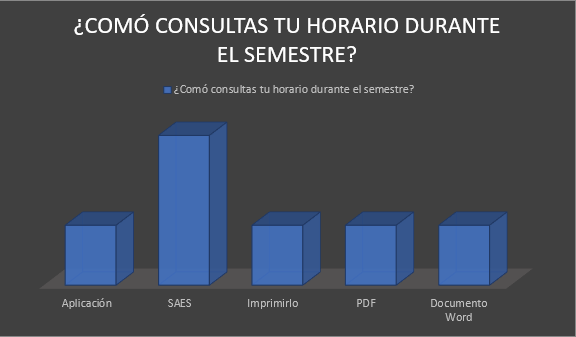
\includegraphics[width=0.7\textwidth]{Imagenes/2.PNG}
    \caption{Medios por los cuales los alumnos consultan su horario. Hemos podido observar que en su mayoría los alumnos acceden al SAES para consultar su horario, dejando otras alternativas en segundo término.}
\label{fig1}
    \end{center}
\end{figure} 
\par\vspace{\baselineskip}
\begin{figure}[H]
    \begin{center}
    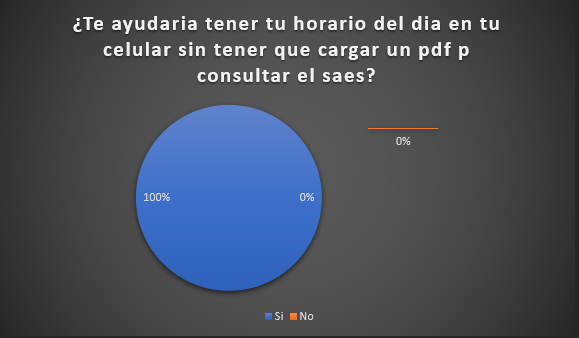
\includegraphics[width=0.7\textwidth]{Imagenes/3.PNG}
    \caption{Muestra de alumnos que preferirían tener su horario de manera más eficiente que en un PDF o consultar el saes para obtener esta información.}
\label{fig1}
    \end{center}
\end{figure} 
\par\vspace{\baselineskip}
\begin{figure}[H]
    \begin{center}
    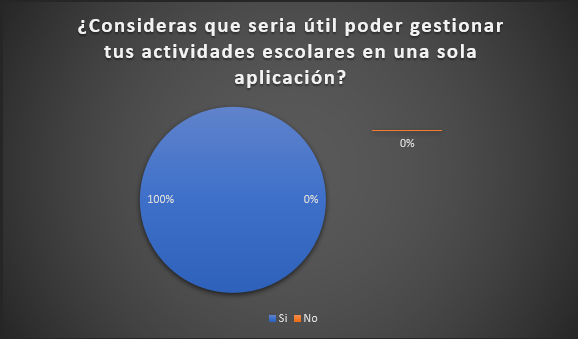
\includegraphics[width=0.7\textwidth]{Imagenes/4.PNG}
    \caption{Muestra de alumnos que preferirían gestionar en una sola aplicación todas sus actividades.}
\label{fig1}
    \end{center}
\end{figure} 
\par\vspace{\baselineskip}
\begin{figure}[H]
    \begin{center}
    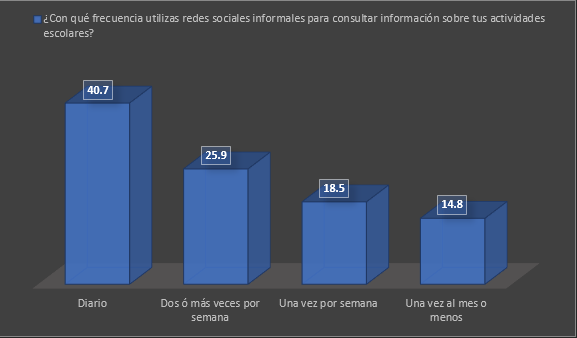
\includegraphics[width=0.7\textwidth]{Imagenes/5.PNG}
    \caption{Muestra de las veces que los alumnos visitan diversas redes sociales para obtener información de sus actividades escolares.}
\label{fig1}
    \end{center}
\end{figure} 
\par\vspace{\baselineskip}
\begin{figure}[H]
    \begin{center}
    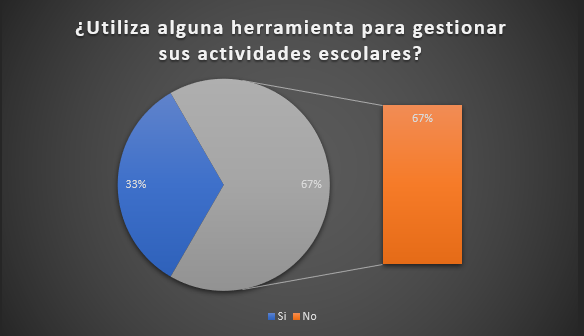
\includegraphics[width=0.7\textwidth]{Imagenes/6.PNG}
    \caption{Muestra de alumnos que sí utilizan herramientas para llevar a cabo la organización de sus actividades.}
\label{fig1}
    \end{center}
\end{figure} 
\par\vspace{\baselineskip}
\begin{figure}[H]
    \begin{center}
    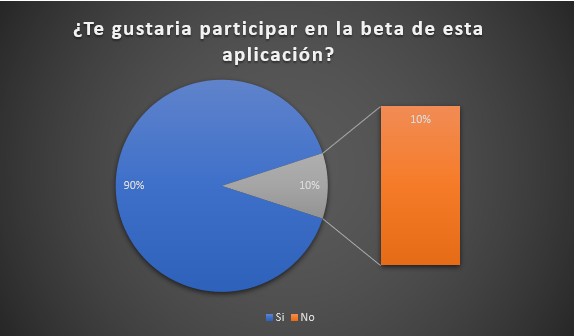
\includegraphics[width=0.7\textwidth]{Imagenes/7.PNG}
    \caption{Versión beta del Sistema. Hemos notado un interés notorio de los alumnos para probar la versión beta de la aplicación. }
\label{fig1}
    \end{center}
\end{figure} 
\par\vspace{\baselineskip}
\begin{figure}[H]
    \begin{center}
    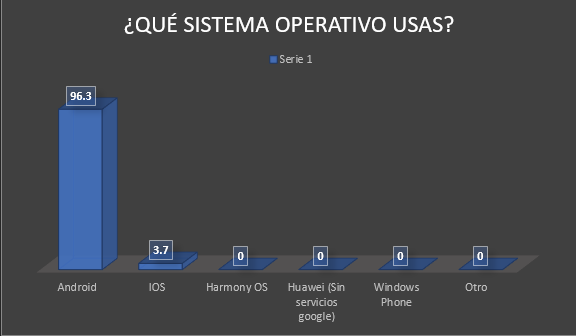
\includegraphics[width=0.7\textwidth]{Imagenes/8.PNG}
    \caption{Versiones de sistema. En esta muestra se ha observado que el 96.3\% corresponde a usuarios del Sistema Operativo Android y el 3.7\% a usuarios que utilizan IOS. }
\label{fig1}
    \end{center}
\end{figure} 

\subsection{Cronograma de actividades}
\justify
Una parte relevante del proyecto ha sido la bitácora de actividades, en ella se ven plasmados los requerimientos iniciales así como los ajustes realizados durante el desarrollo del proyecto, la bitácora nos ayudó a tener un control más adecuado de las actividades a desarrollar. Los requermientos se enlistan con la fecha en la cual se dió inicio.

\centering
\begin{table}[H]
\begin{tabular}{|p{0.6\linewidth}|l |p{0.15\linewidth}|}
\hline
\textbf{Requerimiento}                                   & \textbf{Fecha de inicio} \\ \hline
{Diseños propuestos para Login}                          & Fecha: 31/1/2021 19:30:00 \\ \hline
{Implementación de FingerPrint}                          & Fecha: 18/2/2021 18:43:45 \\ \hline
{Importar el horario del saes leyendo html una vez que el usuario haya iniciado sesión} & Fecha: 28/2/2021 21:00:26 \\ \hline
{Pantalla de ajustes}                                    & Fecha: 28/2/2021 21:01:50   \\ \hline
{Pantalla para ver las tareas mostrando los días en los que hay actividades, al final mostrar que no hay más tareas}                                         &  Fecha: 2/6/2021 0:00:00 \\ \hline
{Pruebsa en el acomodo de imágenes para dar de alta tareas}  &  Fecha: 28/2/2021 23:03:05 \\ \hline
{Color distinto por matera}                               &  Fecha: 8/3/2021 21:54:18 \\ \hline
{Concluir ventana alta de tareas}                           &  Fecha: 15/3/2021 19:02:53 \\ \hline
{Vista de horario como tabla}                            &  Fecha: 15/3/2021 19:24:27 \\ \hline
{Recopilar nombre de las escuelas y enlaces de acceso al saes}    &  Fecha: 21/3/2021 21:52:35  \\ \hline
{Obtener la información del perfil según el mockup desde el saes} &  Fecha: 15/3/2021 19:25:09 \\ \hline
{Pantalla para editar y dar de alta tareas}   &  Fecha: 21/3/2021 23:24:42 \\ \hline
{Vista de detalle por tarea}                    & Fecha: 21/3/2021 23:25:06 \\ \hline
{Dar de alta recordatorios de exámenes ,otros eventos}  & Fecha: 21/3/2021 23:29:38  \\ \hline
{Pantalla de perfil del estudiante}                      &  Fecha: 21/3/2021 23:31:08 \\ \hline
{Exportar horario en PDF}                                &  Fecha: 21/3/2021 23:43:53 \\ \hline

\end{tabular}
\end{table}

\newpage

\centering
\begin{table}[H]
\begin{tabular}{|p{0.6\linewidth}|l |p{0.15\linewidth}|}
\hline
\textbf{Requerimiento}                                   & \textbf{Fecha de inicio} \\ \hline
{Logo de la aplicación}                                  &  Fecha: 21/3/2021 23:48:14 \\ \hline
{Ver las calificaciones desde la aplicación}             &  Fecha: 3/4/2021 1:05:26 \\ \hline
{Pantalla de logros}                                     &  Fecha: 6/4/2021 20:34:12\\ \hline
{Recordatorios 10 minutos antes de cada clase [Android]} &  Fecha: 12/4/2021 23:40:12 \\ \hline
{Pruebas en iOS}                                         &  Fecha: 16/4/2021 18:18:56 \\ \hline
{Widget de tareas [Android]}                             &  Fecha: 16/4/2021 18:20:36 \\ \hline
{Widget de horario [iOS]}                                &  Fecha límite: 23/9/2021 0:00:00 \\ \hline
{Widget de tareas [iOS]}                                 &  Fecha limite: 1/9/2021 0:00:00 \\ \hline
{Recordatorios 10 minutos antes de cada clase [iOS]}     &  Fecha limite: 31/8/2021 0:00:00 \\
\hline 
{Generar app bundle}                                     & Fecha: 20/5/2021 22:08:09  \\ \hline
{Widget de horario [Android]}                            & Fecha limite: 8/6/2021 0:00:00  \\ \hline
{Genrar archivo .ipa}                                    & Fecha: 20/5/2021 22:08:25  \\ \hline
{Esquema de servidor}                                    & Fecha limite: 1/7/2021 0:00:00 \\ \hline
{Menú materia de horario}                                & Fecha limite: 7/7/2021 19:00:00  \\ \hline
{Permitir cambiar el orden de las ventanas}              & Fecha: 20/5/2021 23:14:08  \\ \hline
{Wizard de registro según los cambios descritos en el esquema de servidor} & Fecha limite: 31/7/2021 0:00:00   \\ \hline
{Tema claro y oscuro}              & Fecha limite: 15/7/2021 0:00:00  \\ \hline
{Solicitar permiso formalmente para seguir las reglas de diseño de apple} & Fecha limite: 31/5/2021 0:00:00  \\ \hline
{Compartir tarea, función para compartir las tareas mediante alguna red social}  & Fecha: 23/5/2021 21:21:16 \\ \hline
{Marco teórico}                    & Fecha: 25/5/2021 18:37:25  \\ \hline
{Cuestionario de investigación de mercado}        & Fecha limite: 1/6/2021 3:43:00  \\ \hline
{Video ilustrativo de la funcionalidad básica de la aplicación / Carousel tutorial}  &  Fecha limite: 7/6/2021 22:22:00  \\ \hline
{Mostrar un mensaje cuando no estas inscrito en ninguna materia y permitir actualizar tus datos desdeesa pantalla}                                 & Fecha: 2/7/2021 1:00:25  \\ \hline
{Recordatorios días antes de una tarea [Android]} & Fecha límite: 23/8/2021 0:00:00   \\ \hline
{Recordatorios días antes de la fecha de una tarea}  & Fecha: 4/7/2021 0:32:00  \\ \hline
{Apartado historial de notificaciones}        &  Fecha: 5/7/2021 17:21:06\\ \hline
{Pantalla de información de materia}          &  Fecha limite: 14/7/2021 19:00:00 \\ \hline
{Vista notas de materia}                      &  Fecha limite: 14/7/2021 19:00:00  \\ \hline
{Vista compañeros de grupo}                  & Fecha limite: 14/7/2021 19:00:00  \\ \hline
{Integrar logros [iOS]}                      & Fecha: 7/7/2021 10:06:21  \\ \hline
{Integrar logros [Android]}                  & Fecha: 7/7/2021 10:07:05  \\ \hline
{Vista de valoraciones de materia - profesor}      & Fecha: 11/7/2021 20:16:10  \\ \hline
{Corregir el segmento de tareas y recordatorios en la vista principal}   & Fecha limite: 14/7/2021 19:00:00  \\ \hline
{Posiblidad para agregar el link de los grupos de whatsapp/telegram/webex/teams}  & Fecha: 1/8/2021 19:35:26  \\ \hline
{Ventana de agregar tarea permitir confirmar y guardar una tarea vacía}  & Fecha limite: 9/8/2021 9:00:00  \\ \hline
{Horario de vocacional mismo color,acomodo bugeado } & Fecha limite: 9/8/2021 9:00:00  \\ \hline
{Foto de perfil } & Fecha: 7/8/2021 22:05:03  \\ \hline
{Directorio escolar } & Fecha limite: 23/8/2021 22:20:00  \\ \hline
{Recomendaciones sobre el tamaño de los cuadros de texto } &  Fecha: 9/8/2021 20:06:16\\ \hline
{En algunos casos en el selector de materia solo aperece la primer materia } & Fecha limite: 17/7/2021 19:00:00 \\ \hline
{Todos los enlaces de acerca de... no funciona } & Fecha: 16/8/2021 19:22:42 \\ \hline
{Enlaces de materia fallan al abrir en algunos dispositivos } & Fecha: 16/8/2021 19:24:43 \\ \hline
{Widget de horario falla al iniciar la actividad si la app ya fue terminada } & Fecha: 16/8/2021 19:25:41 \\ \hline
\end{tabular}
\end{table}

\centering
\begin{table}[H]
\begin{tabular}{|p{0.6\linewidth}|l |p{0.15\linewidth}|}
\hline
\textbf{Requerimiento}                                   & \textbf{Fecha de inicio} \\ \hline
{Cambiar de estado una tarea es muy conmfuso entre estados } & Fecha: 16/8/2021 19:30:15 \\ \hline
{Iniciar sesión validar campos } &  Fecha limite: 13/9/2021 22:10:00 \\ \hline
{Botón de nuevo recordatorio no hace nada } & Fecha: 16/8/2021 19:50:18 \\ \hline
{Número de versión no coincide entre acerca de y splashscreen } & Fecha: 16/8/2021 20:00:01 \\ \hline
{EN el carouserl tutorial no se indica qué hacer para avanzar en el tutorial } & Fecha: 16/8/2021 20:06:12 \\ \hline
{La aplicación se cierra al usar la cámara o galería para agergar una imagen a una tarea } & Fecha: 17/8/2021 17:18:29 \\ \hline
{Buscador de profesores por escuela} & Fecha: 17/8/2021 22:11:01 \\ \hline
{Calendario escolar en PDF } & Fecha limite: 23/8/2021 0:00:00 \\ \hline
{Agenda escolar } & Fecha limite: 6/6/2021 18:48:00 \\ \hline
{Mejorar la presentación al compartir una tarea } & Fecha: 4/9/2021 23:11:29 \\ \hline
{Opción en ajustes para presentar las tareas expandidas } & Fecha: 9/9/2021 22:09:38 \\ \hline
{Al cargar la aplicación por primera vez no se muestran las tareas pendientes } & Fecha limite: 27/9/2021 18:03:00 \\ \hline
{Error interno al recuperar un recordatorio } & Fecha limite: 27/9/2021 0:00:00 \\ \hline
{La aplicación inicia en la sección de recordatorios} & Fecha: 12/9/2021 20:49:33  \\ \hline
{Solicita el permiso de almacenamiento después de generar el PDF } & Fecha: 12/9/2021 20:56:03 \\ \hline
{Error en el compresor de imágenes capturadas por la cámara } & Fecha: 12/9/2021 21:06:08  \\ \hline
{Al completar los recordatorios no desaparecen de la lista } & Fecha: 12/9/2021 21:23:48 \\ \hline
{Cuando se agrega un contacto que tiene solamente correo no da el acceso para enviarlo } & Fecha: 12/9/2021 21:39:35 \\ \hline
{Recuperar enlaces oficiales de todas las instituciones soportadas } & Fecha: 12/9/2021 21:45:03 \\ \hline
{Solocotar característica, reportar bug solo funciona si tiene una cuenta logueada } & Fecha: 12/9/2021 22:07:31  \\ \hline
{Integrar plantilla en correo soporte } & Fecha: 12/9/2021 22:08:42 \\ \hline
{Permitir ocultar nombre de información de materia } & Fecha limite: 27/9/2021 0:00:00 \\ \hline
{Editar Popup para cambiar foto de perfil } & Fecha limite: 20/9/2021 23:00:00 \\ \hline
\end{tabular}
\end{table}
%%%%%%%%%%%%%%%%%%%%%%%%%%%%%%%%%%% TABLA 1 %%%%%%%%%%%%%%%%%%%%%%%%%%%%%%%%%%%%%%%%%%%%%%
\begin{table}[ht]
\centering
\begin{tabular}{|l |l |l |l |l |}
\hline
\multicolumn{3}{|c|}{\textbf{Aplicación móvil}} \\
\hline
\centering\textbf{Plataforma} & {Android} & {iOS} \\ \hline
\centering\textbf{Versión mínima} & {API 23+ 6.0.1 Marshmallow} & {iOS 9} \\ \hline
\centering\textbf{Versión destino} & {API 30 Honeycomb} & {iOS 14.5} \\ \hline
\centering\textbf{Procesador} & {arm64\-v8a, armeabi\-v7a, x86\_64} & {A9, A10, A11, A12} \\ \hline
\centering\textbf{Hardware} & {Dispositivos móviles y tabletas Android} & {Dispositivos móviles iOS}  \\ \hline
\end{tabular}
\end{table}
%%%%%%%%%%%%%%%%%%%%%%%%%%%%%%%%%%% TABLA 2 %%%%%%%%%%%%%%%%%%%%%%%%%%%%%%%%%%%%%%%%%%%%%%
\begin{table}[H]
\begin{center}
\begin{tabular}{| l | l |}
\hline
\textbf{Componente} & \textbf{Origen} \\ \hline
Conectividad a internet & Requerido \\
Cámara & Deseable opcional \\ \hline
\end{tabular}
\end{center}
\end{table}
%%%%%%%%%%%%%%%%%%%%%%%%%%%%%%%%%%% TABLA 3 %%%%%%%%%%%%%%%%%%%%%%%%%%%%%%%%%%%%%%%%%%%%%%
\begin{table}[H]
\centering
\begin{tabular}{|l |l |l |l |l |}
\hline
\multicolumn{5}{|c|}{\textbf{Proveedor de base de datos}} \\
\hline
\centering\textbf{Version SQL} & \textbf{CPU} & \textbf{RAM} & \textbf{Almacenamiento} & \textbf{Tipo de almacenamiento} \\ \hline
\centering{Sqlserver express 14.00.3356.20.v1} & {1} & {1Gb} & {20 Gbs} & {SSD} \\ \hline
\hline
\multicolumn{5}{|c|}{\textbf{Proveedor de servicios web}} \\
\hline
\centering\textbf{Entorno} & \textbf{CPU} & \textbf{RAM} & \textbf{Almacenamiento} & \textbf{Tipo de almacenamiento} \\ \hline
\centering{.NET Core 3.1 (C\#/PowerShell)} & {1} & {512 Mb} & {50 Gbs} & {SSD} \\ \hline
\end{tabular}
\end{table}
\newpage
%%%%%%%%%%%%%%%%%%%%%%%%%%%%%%%%%%%%%%%%% Requerimientos funcionales 


\begin{longtable}{|p{0.2\linewidth}|p{0.2\linewidth}|p{0.1\linewidth}|p{0.4\linewidth}|}
\hline
\textbf{Requerimiento} & \textbf{Descripción} & \textbf{Prioridad} & \textbf{Acciones iniciadoras y comportamiento esperado} \\ \hline

Protección biométrica  & Uso del sistema biométrico por huella para protección de la aplicación & Medio     & Una vez que el usuario tiene su registro puede activar la opción de ingreso por huella  \\\hline

Visualizar horario     & Visualización de horario actual ordenado por clase y colores           & Alto      & Al ingresar al apartado de horario se desplegará una pantalla el cual lo contendrá  \\\hline

Generar horario en pdf & Se obtiene una versión PDF del horario                                 & Alto      & Al  el botón para generar horario en automático se tendrá la opción para guardarlo o compartirlo \\\hline

{Generar horario en pdf} & {Se obtiene una versión en PDF del horario} & {Alto} & {Al presionar en la opción para generar horario en automático se tendrá la opción para guardarlo o compartirlo} \\ \hline

{Consulta calificaciones} & {Visualizar las calificaciones y actualizar las mismas} & {Alto} & {Al ingresar al botón de calificaciones se mostrarán las más recientes, se pueden actualizar las calificaciones presionando el botón actualizar} \\ \hline

{Consulta información escolar} & {Al ingresar por primera vez se podrá visualizar la información del alumno como carrera, escuela y avance escolar} & {Alto} & {Ingresar a la opción perfil de usuario} \\ \hline

{Crea tareas} & {Creación de tareas por materia con título, descripción, fecha de inicio y fin, así como adjuntar imágenes} & {Alto} & {Ingresar al botón crear tareas se desplegará una pop-up para llenar los campos, una vez creada aparecerá en la pantalla principal en orden de fecha de expiración junto con otras tareas} \\ \hline

{Crea recordatorios} & {Creación de recordatorios por materia con título, descripción, fecha de inicio y fin} & {Alto} & {Ingresar al botón crear recordatorio se desplegará un pop up para llenar los campos, una vez creada aparecerá en la pantalla principal de recordatorios en orden de fecha de expiración} \\ \hline

{Compartir enlaces} & {Compartir tareas mediante un enlace que se puede compartir} & {Alto} & {En la tarea, presionar el botón compartir el cual generará un link} \\ \hline

{Compartir tareas} & {Compartir tareas mediante un enlace que se puede compartir} & {Alto} & {En la tarea, presionar el botón compartir el cual generará un link} \\ \hline

{Widget de tareas} & {Visualización de tareas en un widget} & {Alto} & {Despliega widget mediante el un gesto en el dispositivo} \\ \hline

{Notificaciones 15 minutos antes de clase} & {Recibe notificaciones 15 minutos previos al inicio de cada clase} & {Alto} & {Las notificaciones se desplegarán en automático en la barra de notificaciones} \\ \hline

{Notificaciones de tarea} & {Recibe notificaciones de tareas próximas a vencer} & {Alto} & {Las notificaciones se desplegarán en automático en la barra de notificaciones la barra de notificaciones} \\ \hline

{Adjuntar imágenes en tareas} & {Al crear una tarea se pueden adjuntar imágenes desde la galería o cámara fotográfica} & {Alto} & {En la opción crear tareas, el botón adjuntar imagen desplegará una la opción para adjuntar imágenes desde la cámara o galería del equipo} \\ \hline

{Información por materia} & {Se desplegará información relevante sobre la materia como el grupo y la clase a tomar, así como un foro para estudiantes para discutir temas de la clase así cómo saber qué alumnos están inscritos en ella (compañeros de clase)} & {Alto} & {Al presionar una materia en el horario se desplegará una pop-up la cual brindará la opción de información por materia, así como la opción de ingresar al foro o compañeros de clase} \\ \hline

{Muro de tareas y recordatorios} & {La pantalla principal muestra las tareas y recordatorios ordenados por orden de importancia (fecha a expirar)} & {Alto} & {Al iniciar sesión en la aplicación será primer pantalla a visualizar} \\ \hline
\end{longtable}
%%%%%%%%%%%%%%%%%%%%%%%%%%%%%%%%%%%%%%%%%%%%%%%%%%%%%%%%%%%%%%%%%%%%%
\justify
\subsection{Implementacion de ISO 2000 en el proyecto}
\justify
ISO 2000
En base a la ISO 2000 se deben desarrollar los siguientes pasos:\\
\begin{itemize}
\item Evaluar necesidades y metas de organización:\\
Se evaluaron las necesidades de los alumnos de la carrera de computación y la necesidad más grande fue la falta de organización en las tareas cotidianas escolares y la meta a desarrollo es una aplicación para poder administrar sus actividades escolares.
\item Obtener información:\\
Se realizaron encuesta a los alumnos de la carrera de computación para saber el uso cotidiano del celular y su forma de organizar sus actividades escolares.
\item Nombrar consultor:\\
Profesor Oscar Cruz García quien nos ha ayudado en la estructuración de las partes del proyecto.
\item Toma de conciencia y formación:\\
a) La protección de los datos sensibles de los usuarios\\
b) Los objetivos de calidad pertinentes para el proyecto\\
c) La contribución que haremos a los alumnos y beneficios que mejoraran el desempeño de ellos.\\
d) Y también lo que implica incumplir los requisitos del Sistema proyecto.
\item Análisis de brech:\\
Evaluamos las diferencias entre el desempeño real que tendrá el proyecto y el desempeño esperado que teníamos al inicio de este.
\item Revisión o definición de procesos:\\
¨ Se hizo un análisis de los requerimientos.\\
¨ Se diagnosticaron los requerimientos funcionales y no funcionales.\\
¨ Formación de las etapas de implementación de los requerimientos.\\
¨ Verificación de los estándares de calidad que debe tener le proyecto.
\item Suministrar personal:\\
Se organizaron las tares entre los integrantes del equipo para así tener un mayor desempeño en el desarrollo.\\
Establecer cronograma:\\
Al ya tener definidos los alcances del proyecto se implementó el cronograma de actividades utilizando Trello para llevar una organización de ellas.
\end{itemize}
\subsection{Diagrama de Casos de Uso}
\begin{figure}[H]
    \begin{center}
    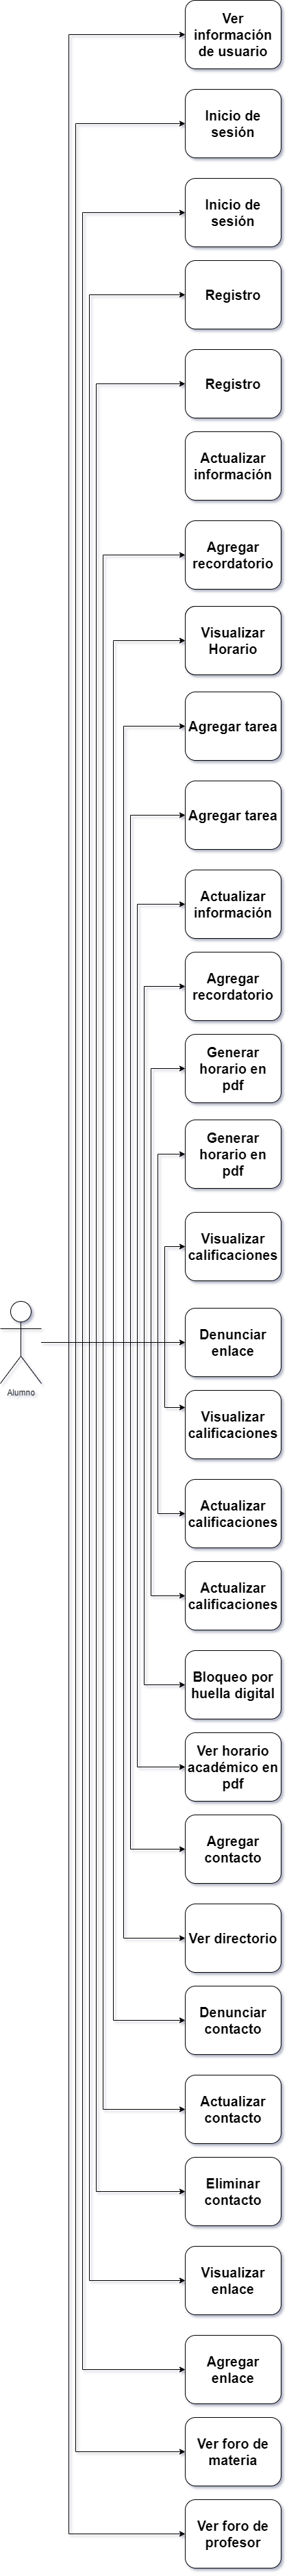
\includegraphics[width=0.13\textwidth]{Imagenes/SOE_CASOSDEUSO.PNG}
    \caption{Diagrama de casis de uso entre la aplicación y el alumno.}
\label{fig1}
    \end{center}
\end{figure} 


\newpage
\subsection{Matriz de trazabilidad de casos de uso.}


\begin{table}[ht]
\begin{center}
\begin{tabular}{|p{0.6\linewidth}|c |p{0.15\linewidth}|}
\hline                                                   & Actor: Alumno \\ \hline
{CUS1: Ver información de usuario}                       &  x \\ \hline
{CUS2: Inicio de sesión}                                 &    \\ \hline
{CUS3: Registro}                                         &  x \\ \hline
{CUS4: Actualizar información}                           &    \\ \hline
{CUS5: Agregar tarea}                                    &  x \\ \hline
{CUS6: Agregar recordatorio}                             &  x \\ \hline
{CUS7: Visualizar horario}                               &  x \\ \hline
{CUS8: Generar horario en PDF}                           &  x \\ \hline
{CUS9: Visualizar calificaciones}                        &  x \\ \hline
{CUS10: Actualizar calificaciones}                       &    \\ \hline
{CUS11: Activar / desactivar bloqueo por huella digital} &  x \\ \hline
{CUS12: Activar / desactivar barra lateral de horario}   &  x \\ \hline
{CUS13: Ver horario académico en PDF}                    &  x \\ \hline
{CUS14: Ver directorio}                                  &  x \\ \hline
{CUS15: Agregar contacto}                                &  x \\ \hline
{CUS16:  Denunciar contacto}                             &  x \\ \hline
{CUS17: Actualizar contacto}                             &  x \\ \hline
{CUS18: Eliminar contacto}                               &  x \\ \hline
{CUS19: Visualizar enlace}                               &    \\ \hline
{CUS20: Agregar enlace}                                  &  x \\ \hline
{CUS21: Denunciar enlace}                                &  x \\ \hline
{CUS22: Ver foro de comunidad}                           &  x \\ \hline
{CUS23: Ver foro de profesor}                            &  x \\ \hline
{CUS24: Ver calendario escolar}                          &  x \\ \hline
{CUS25: Mantener expandidas las tareas}                  &  x \\
\hline 
\end{tabular}
\end{center}
\end{table}

\justify
En donde: \\ 
\textbf{\\}
\textbf{CUS:} Hace referencia al caso de uso \\
\textbf{Usuario:} El actor dentro de esta matríz de trazabilidad.


\newpage
\subsection{Matriz de trazabilidad}
\noindent
\begin{longtable}{|p{0.3cm}|p{0.11\linewidth}|p{0.07\linewidth}|p{0.04\linewidth}|p{0.08\linewidth}|p{0.14\linewidth}|p{0.13\linewidth}|p{0.1\linewidth}|p{0.12\linewidth}|}
%\begin{table}
 % \begin{tabular} {|p{0.3cm}|p{0.12\linewidth}|p{0.09\linewidth}|p{0.05\linewidth}|p{0.09\linewidth}|p{0.14\linewidth}|p{0.14\linewidth}|p{0.1\linewidth}|p{0.13\linewidth}|}
    \hline
    ID & REQUISITO                                  & TIPO        & PRIO  & ESTADO     & OBJETIVO                                                                                                                                                                                                                                & ENTREGABLE                               & ESTADO     & VALIDACIÓN               \\ \hline
    1  & Protección   biométrica                    & Android/ IOS & Alta  & Finalizado & Uso del sistema biométrico por huella para   protección de la aplicación.                                                                                                                                                               & Desbloqueo   de la aplicación con biometría & Testing    & 17 de ago. a las 20:05   \\ \hline
    2  & Visualizar horario                         & Saes        & Alta  & Finalizado & Visualización de horario actual ordenado por   clase y colores                                                                                                                                                                          & Horario Obtenido del saes                   & Completado & 28 de mar. a las 22:59   \\ \hline
    3  & Exportar horario en PDF                    & Research    & Media & Finalizado & Generar el horario en formato PDF                                                                                                                                                                                                       & Se obtiene una versión en PDF del horario   & Completado & 6 de abr. a las 20:28    \\ \hline
    4  & Pantalla   de perfil del estudiante        & Diseño      & Alta  & Finalizado & Al ingresar por primera vez se   podrá visualizar la información del alumno como carrera, escuela y avance   escolar                                                                                                                    & Venta perfil de estudiante                  & Completado & 17 de ago. a las 20:04   \\ \hline
    5  & Widget   de horario                        & Android     & Alta  & Finalizado & Desarrollo de widget de horario   orientado a Android                                                                                                                                                                                   & Widget de horario [Android]                 & Completado & 08 de jun. a   las 00:00 \\ \hline
    6  & Esquema   de servidor                      & API         & Alta  & Finalizado & Una iniciativa para eliminar el procesamiento   en el dispositivo de cliente y apostar por una arquitectura más segura                                                                                                                  & API                                         & Completado & 01 de jul. a las 00:00   \\ \hline
    7  & Crea   recordatorios                       & Page        & Alta  & Finalizado & Creación de recordatorios por   materia con título, descripción, fecha de inicio y fin                                                                                                                                                  & Lamba AWS Cloud clusters                    & Completado & 17 de ago. a las 20:04   \\ \hline
    8  & Crea   tareas                              & Page        & Alta  & Finalizado    & Creación de tareas por materia con   título, descripción, fecha de inicio y fin, así como adjuntar imágenes                                                                                                                             & Ventana de altas                            & Testing    & 17 de ago. a las 20:05   \\ \hline
    9  & Consulta   calificaciones                  & Saes        & Alta  & Finalizado    & Visualizar las calificaciones y   actualizar las mismas                                                                                                                                                                                 & Ventana de calificaciones                   & Testing    & 17 de ago. a las 20:05   \\ \hline
    10 & Widget de tareas [Android]                 & Android     & Alta  & Finalizado & Desarrollo de widget de tareas   orientado a Android                                                                                                                                                                                    & Widget de tareas [Android]                  & Testing    & 17 de ago. a   las 20:05 \\ \hline
    11 & Compartir   Tarea                          & API/ Diseño  & Alta  & Finalizado    & Se pueden adjuntar enlaces de   interés para un grupo de clase                                                                                                                                                                          & Compartir   enlaces                         & Testing    & 17 de ago. a las 20:05   \\ \hline
    13 & Notificaciones   10 minutos antes de clase & Research    & Alta  & Finalizado     & Función para compartir las tareas                                                                                                                                                                                                       & Compartir tarea                             & Testing    & 17 de ago. a las 20:05   \\ \hline
    12 & Compartir   enlaces                        & API/ Diseño  & Alta  & Finalizado   & Recibe notificaciones 10 minutos   previos al inicio de cada clase                                                                                                                                                                      & Recordatorios 10 minutos                    & Testing    & 17 de ago.   a las 20:05 \\ \hline
    14 & Notificaciones   de tarea                  & Research    & Alta  & Finalizado    & Recibe notificaciones de tareas   próximas a vencer                                                                                                                                                                                     & Recordatorios por tarea                     & Testing    & 17 de ago. a las 20:05   \\ \hline
    15 & Adjuntar   imágenes en tareas              & Page        & Alta  & Finalizado & Al crear una tarea se pueden   adjuntar imágenes desde la galería o cámara fotográfica                                                                                                                                                  & Actualización ventana de altas              & Testing    & 17 de ago.   a las 20:05 \\ \hline
    16 & Información por materia                    & Page        & Alta  & Finalizado & Se desplegará información relevante   sobre la materia como el grupo y la clase a tomar, así como un foro para estudiantes   para discutir temas de la clase así cómo saber qué alumnos están inscritos en   ella (compañeros de clase) & Actualización ventana de altas              & Testing    & 17 de ago. a las 20:05   \\ \hline
    17 & Muro   de tareas y recordatorios           & Page        & Alta  & Finalizado & La pantalla principal muestra las   tareas y recordatorios ordenados por orden de importancia (fecha a expirar)                                                                                                                         & Actualización ventana de altas              & Testing    & 17 de ago.   a las 20:05 \\ \hline
    \end{longtable}
%\end{table}
  


\subsection{Diagrama de funcionamiento}
\begin{figure}[H]
    \begin{center}
    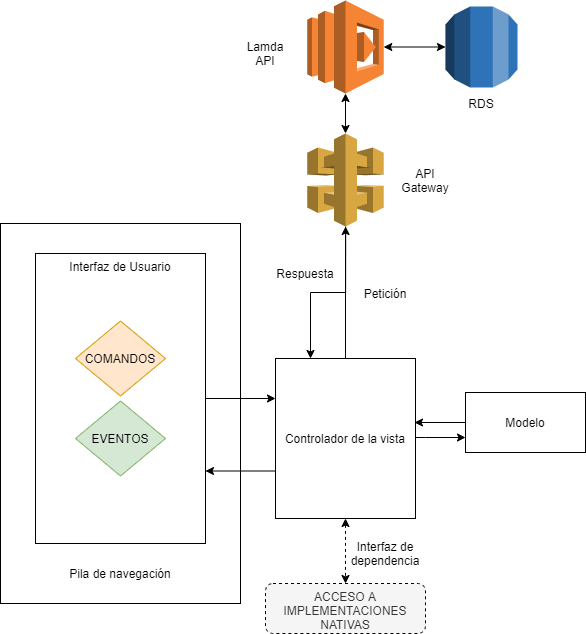
\includegraphics[width=1\textwidth]{Imagenes/11.PNG}
    \caption{Funcionamiento general de la aplicación y su comunicación con la nube.}
\label{fig1}
    \end{center}
\end{figure} 
\subsection{Modelo de  solución de software}
\begin{figure}[H]
    \begin{center}
    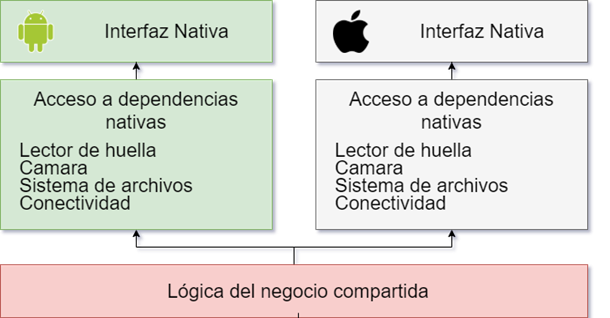
\includegraphics[width=0.8\textwidth]{Imagenes/12.PNG}
    \caption{Modelo de arquitectura interna de la solución multiplataforma.}
\label{fig1}
    \end{center}
\end{figure} 

\subsection{Diagrama de funcionamiento ventana principal}
\begin{figure}[H]
    \begin{center}
    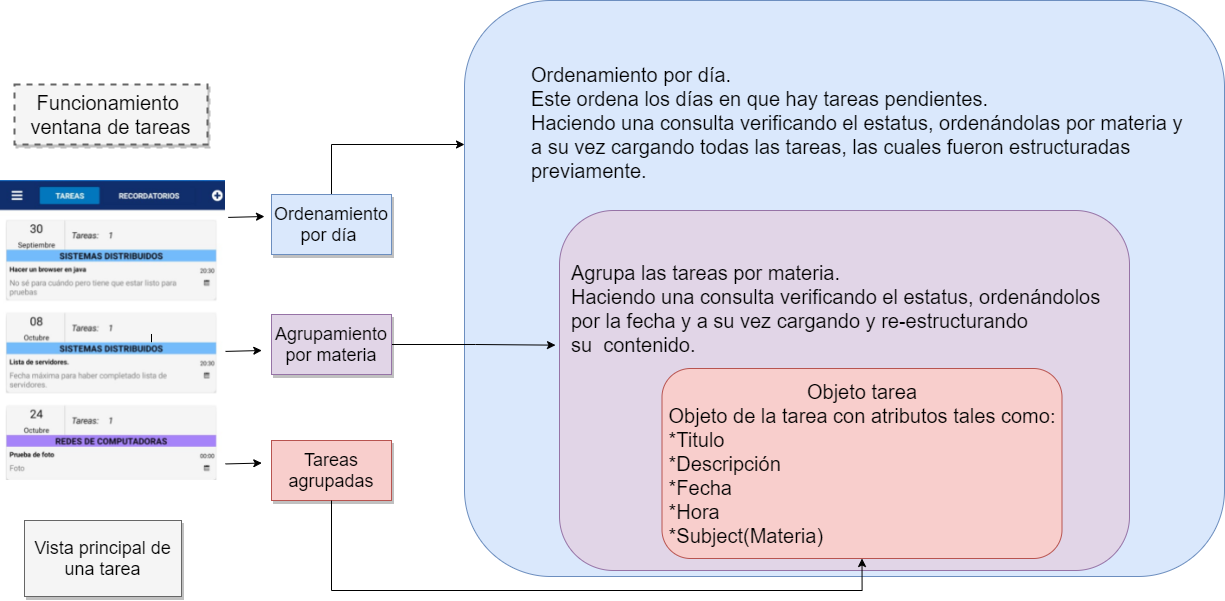
\includegraphics[width=0.8\textwidth]{Imagenes/DiagramaTareas.png}
    \caption{Esquema de la estructura de la ventana de tareas}
\label{fig1}
    \end{center}
\end{figure} 
\begin{landscape}
\subsection{Diagrama entidad-relación}
\begin{figure}[h]
\centering
    \begin{center}
    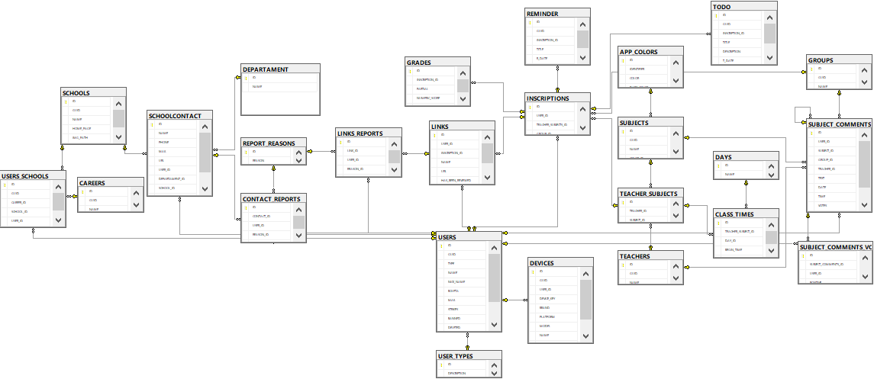
\includegraphics[width=1.3\textwidth]{Imagenes/diagrama.png}
    \caption{Diagrama entidad-relación de la base de datos alojada en el servicio web.}
\label{fig1}
    \end{center}
\end{figure} 
\end{landscape}
\newpage
\subsection{Desarrollo de API}
\begin{figure}[H]
    \begin{center}
    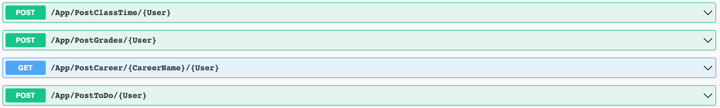
\includegraphics[width=0.8\textwidth]{Imagenes/api.png}
    \caption{Ejemplos de verbos modificadores y recuperadores de el API}
\label{fig1}
    \end{center}
\end{figure} 
\begin{figure}[H]
    \begin{center}
    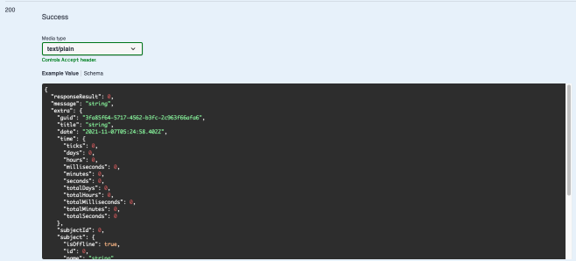
\includegraphics[width=0.8\textwidth]{Imagenes/api2.png}
    \caption{Ejemplo de respuesta del verbo modificador "ShareTodo"}
\label{fig1}
    \end{center}
\end{figure} 
\subsection{Llamada desde la aplicación al API}
\begin{figure}[H]
    \begin{center}
    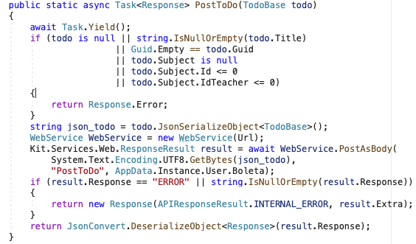
\includegraphics[width=0.8\textwidth]{Imagenes/api3.png}
    \caption{Fragmento de código de la llamada desde la aplicación a el servicio Web}
\label{fig1}
    \end{center}
\end{figure} 
\begin{figure}[H]
    \begin{center}
    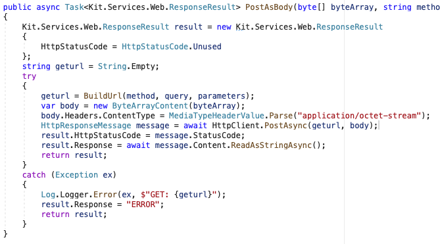
\includegraphics[width=0.8\textwidth]{Imagenes/api4.png}
     \caption{Fragmento de código de las llamada POST}
\label{fig1}
    \end{center}
\end{figure} 
\subsection{Fragmento de código de la pantalla para dar de alta una tarea}
\begin{figure}[H]
    \begin{center}
    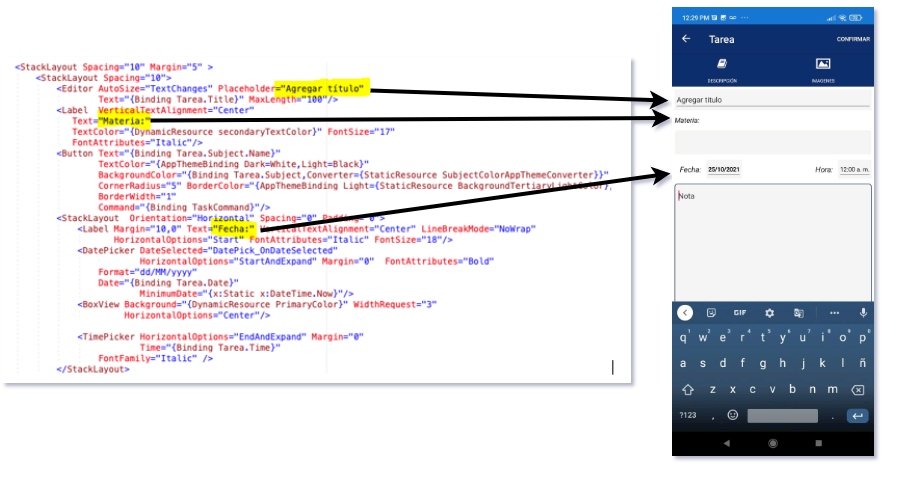
\includegraphics[width=1\textwidth]{Imagenes/tareas.png}
    \caption{Fragmento de código del maquetado de la interfaz gráfica en la pantalla para dar de alta una tarea}
\label{fig1}
    \end{center}
\end{figure} 

\subsection{Implementación widget nativo}
\begin{figure}[H]
    \begin{center}
    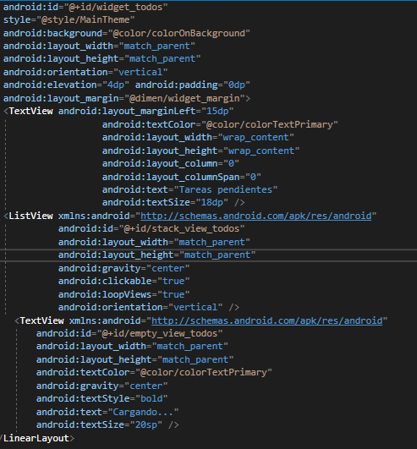
\includegraphics[width=0.8\textwidth]{Imagenes/widget.png}
    \caption{Fragmento de código de la interfaz gráfica del widget nativo para Android.}
\label{fig1}
    \end{center}
\end{figure} 
\begin{figure}[H]
    \centering
    \subfloat[\centering Widget de tareas]{{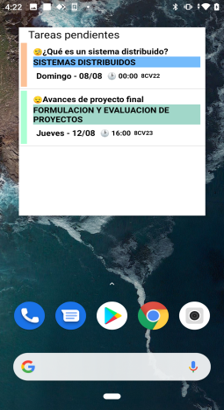
\includegraphics[height=12cm]{Imagenes/widget1} }}%
    \qquad
    \subfloat[\centering Widget de horario]{{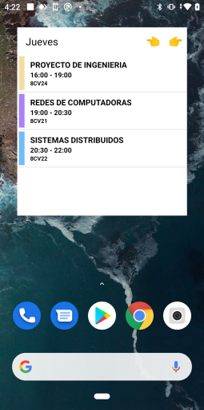
\includegraphics[height=12cm]{Imagenes/widget2} }}%
    \caption{Widget nativo (Andorid)}%
    \label{fig:example}%
\end{figure}
\newpage

\subsection{Principales funcionalidades de la aplicación.}
\begin{figure}[ht!]% 
  \begin{minipage}[b]{0.49\linewidth}%
    \centering
    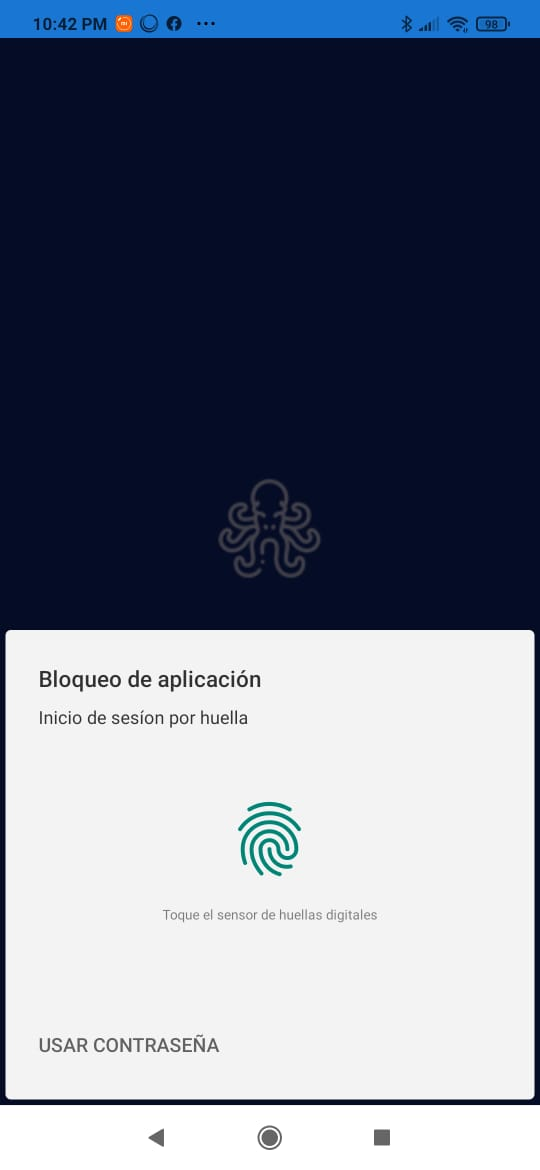
\includegraphics[width=.4\linewidth]{Imagenes/SOE1.jpeg} %
    \caption{En el inicio de sesión se despliega la \\ opción para ingresar por medio de huella,\\ alternativamente por contraseña.}%
  \end{minipage}%%
  \vspace{1cm}%
  \begin{minipage}[b]{0.49\linewidth}
    \centering
    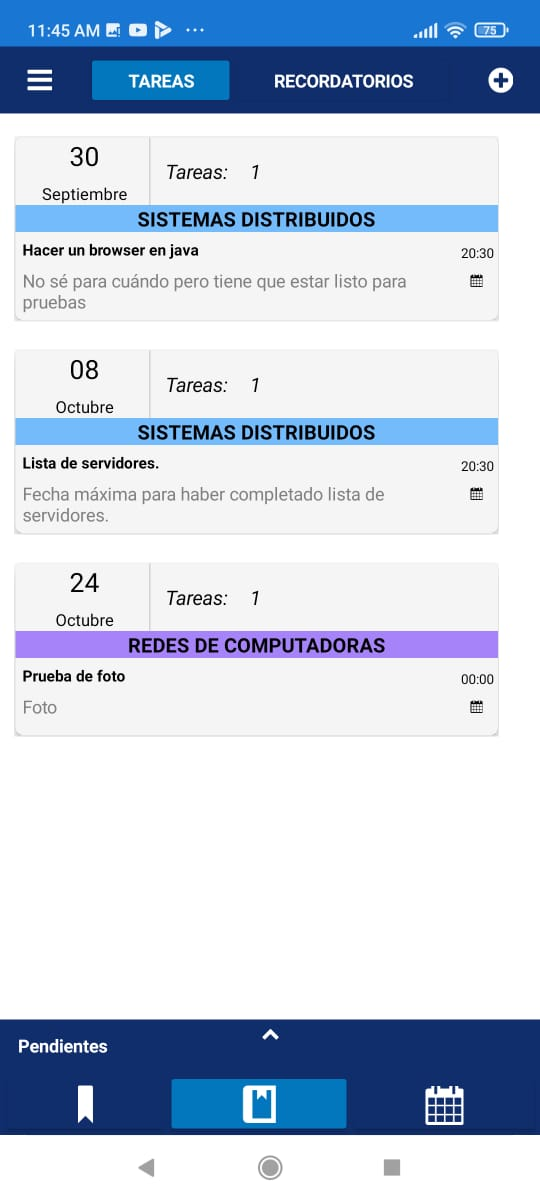
\includegraphics[width=.4\linewidth]{Imagenes/SOE2.jpeg} 
    \caption{La pantalla de tareas es la primera en mostrarse una vez que se ingresa a la aplicación.} 
  \end{minipage} %
  \vspace{1cm}%
  \begin{minipage}[b]{0.49\linewidth}
    \centering
    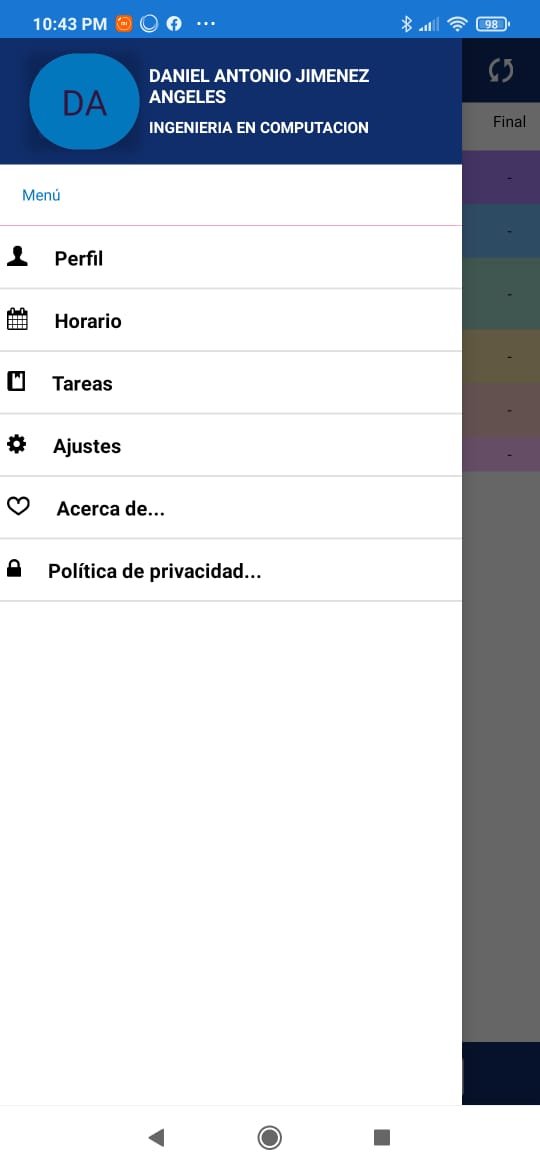
\includegraphics[width=.4\linewidth]{Imagenes/SOE3.jpeg} 
    \caption{En esta pantalla de muestran los\\ siguientes submenús: Perfil, horario, tareas,\\ ajustes, aderca de y política de privacidad.} 
  \end{minipage}%% 
  \vspace{1cm}%
  \begin{minipage}[b]{0.49\linewidth}%
    \centering%
    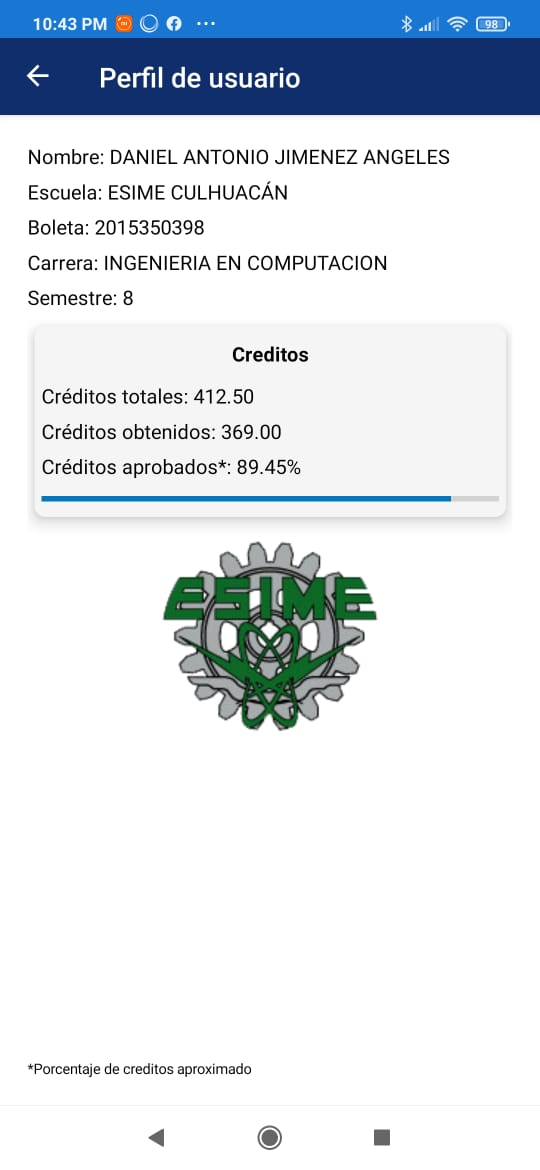
\includegraphics[width=.4\linewidth]{Imagenes/SOE4.jpeg} %
    \caption{Ingresando a la opción perfil
se muestran datos del alumno: Nombre, Escuela, Boleta, Carrea, Semestre, Créditos totales, Créditos obtenidos, Créditos aprobados*.}%
  \end{minipage}% 
  \vspace{1cm}%
\end{figure}%
%
\newpage

\begin{figure}[ht!] 
  \begin{minipage}[b]{0.49\linewidth}
    \centering
    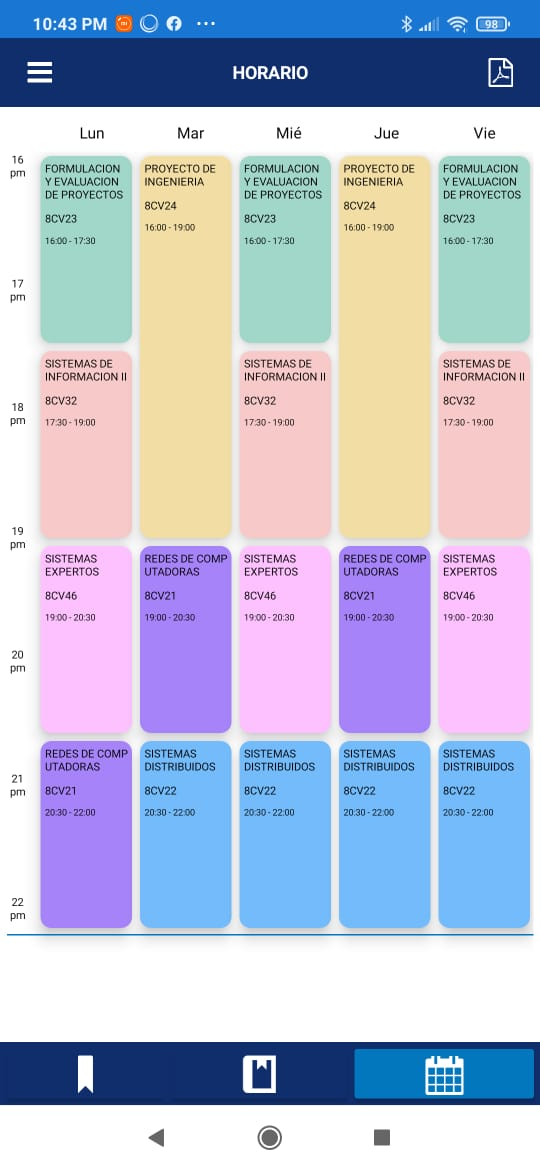
\includegraphics[width=.4\linewidth]{Imagenes/SOE5.jpeg} 
    \caption{En el inicio de sesión se despliega la \\ opción para ingresar por medio de huella,\\ alternativamente por contraseña.}
  \end{minipage}%%
  \vspace{1cm}
  \begin{minipage}[b]{0.49\linewidth}
    \centering
    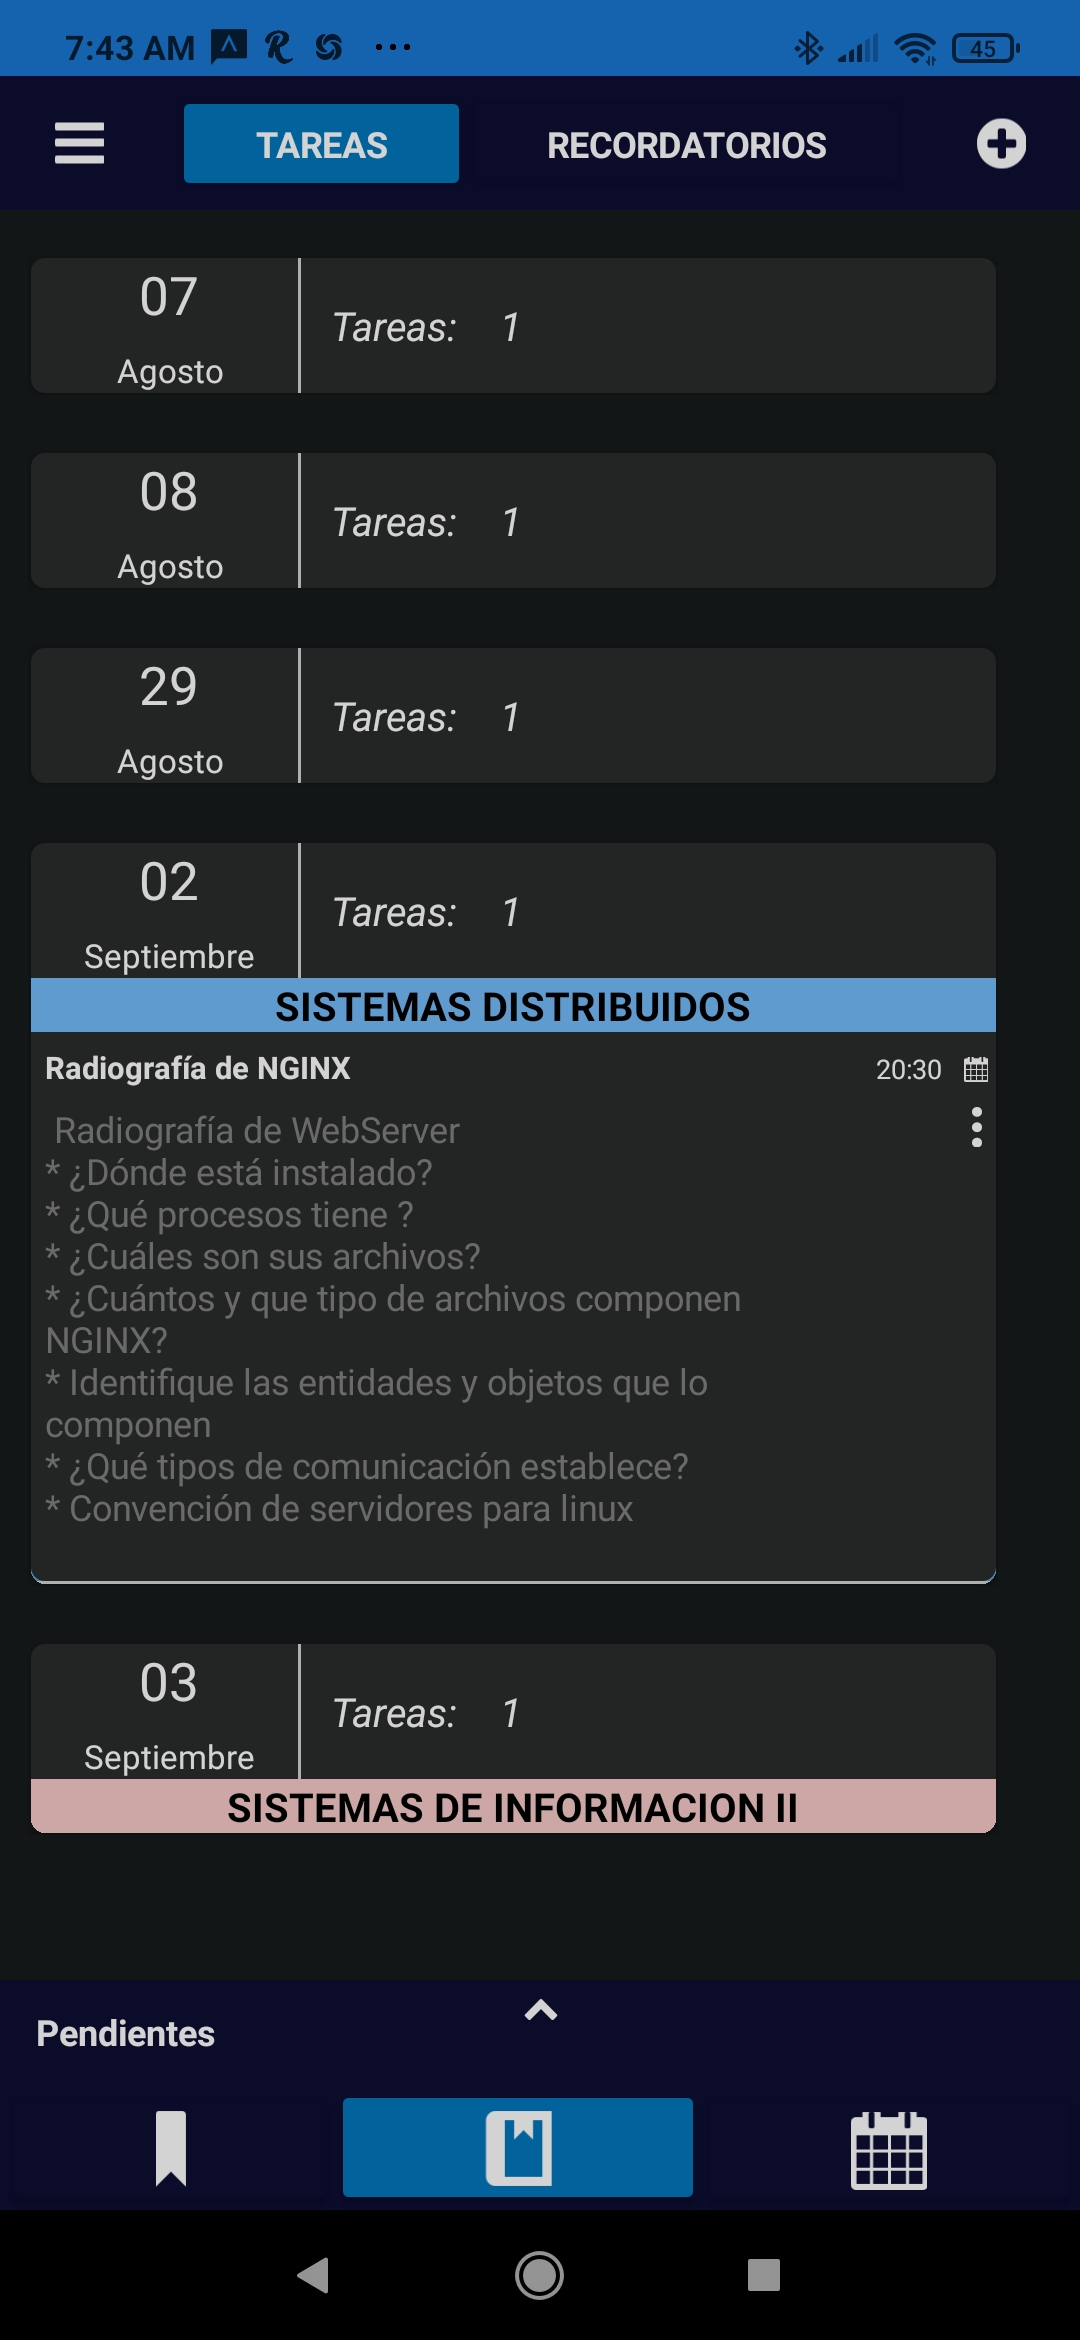
\includegraphics[width=.4\linewidth]{Imagenes/SOE6.jpg} 
    \caption{La pantalla de tareas es la primera en mostrarse una vez que se ingresa a la aplicación.} 
  \end{minipage} 
  \vspace{1cm}
  \begin{minipage}[b]{0.49\linewidth}
    \centering
    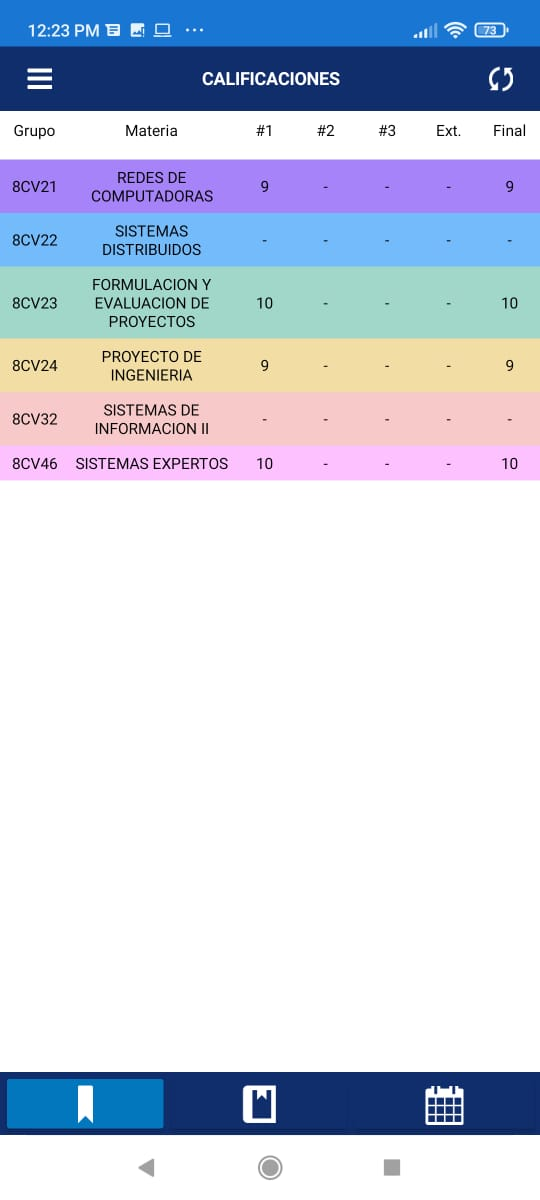
\includegraphics[width=.4\linewidth]{Imagenes/SOE7.jpeg} 
    \caption{En esta pantalla de muestran los\\ siguientes submenús: Perfil, horario, tareas,\\ ajustes, aderca de y política de privacidad.} 
  \end{minipage}%% 
  \vspace{1cm}
  \begin{minipage}[b]{0.49\linewidth}
    \centering
    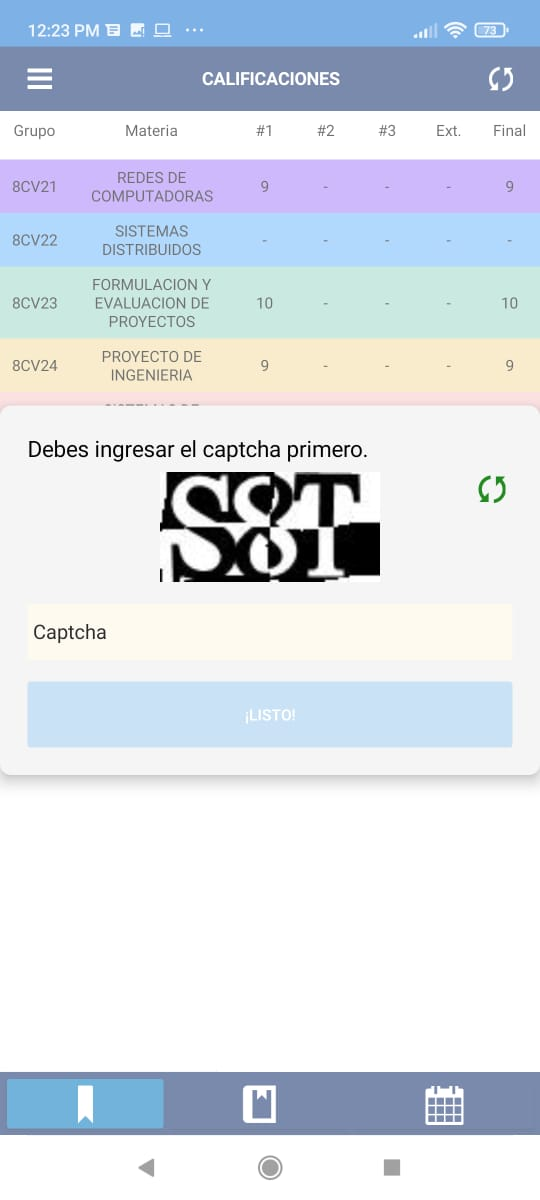
\includegraphics[width=.4\linewidth]{Imagenes/SOE8.jpeg} 
    \caption{Ingresando a la opción perfil
se muestran datos del alumno: Nombre, Escuela, Boleta, Carrea, Semestre, Créditos totales, Créditos obtenidos, Créditos aprobados*.} 
  \end{minipage} 
  \vspace{1cm}
\end{figure}

\newpage

\begin{figure}[ht!] 
  \begin{minipage}[b]{0.49\linewidth}
    \centering
    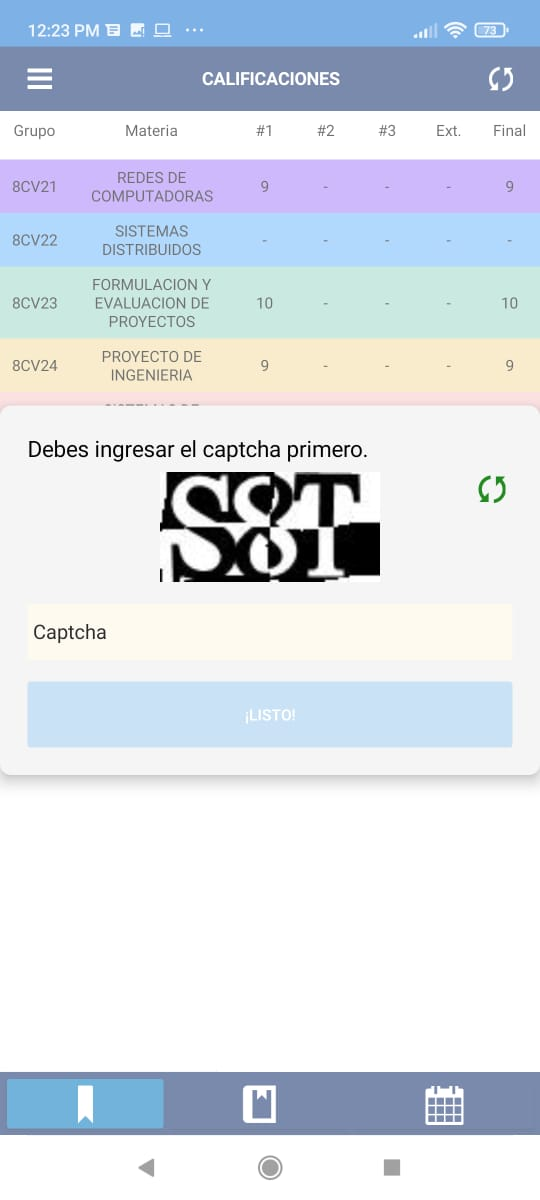
\includegraphics[width=.4\linewidth]{Imagenes/SOE8.jpeg} 
    \caption{Una vez resuelto el captcha\\ las calificaciones se actualizan en automático.}
  \end{minipage}%%
  \vspace{1cm}
  \begin{minipage}[b]{0.49\linewidth}
    \centering
    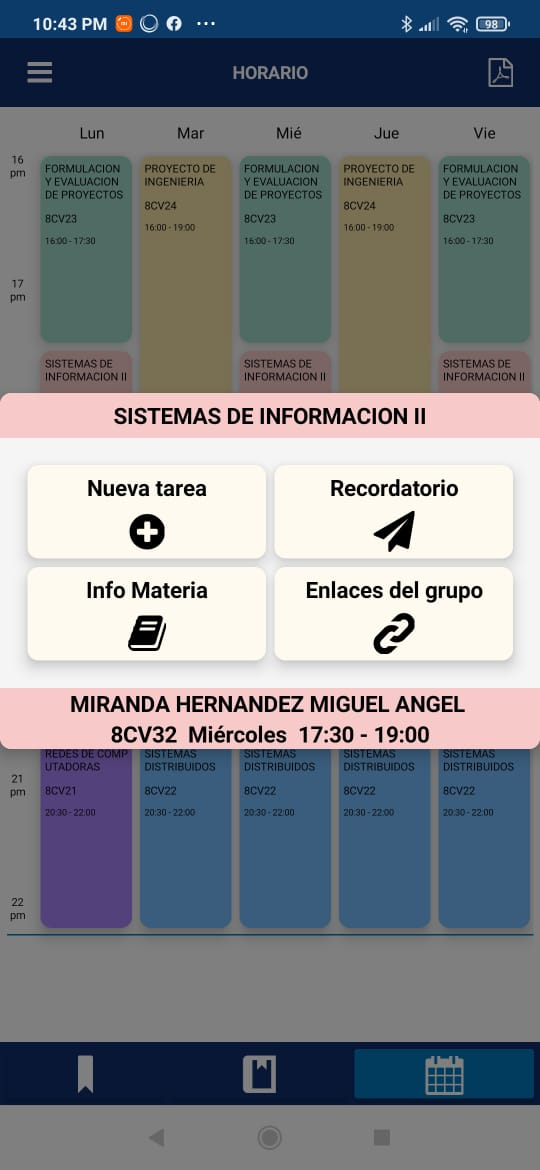
\includegraphics[width=.4\linewidth]{Imagenes/SOE9.jpeg} 
    \caption{La pantalla de horario muestra las clases inscritas con dos ejes de referencia; los días de la semana de lunes a viernes y un rango de horas desde el inicio hasta el fin de clases en el día.} 
  \end{minipage} 
  \vspace{1cm}
  \begin{minipage}[b]{0.49\linewidth}
    \centering
    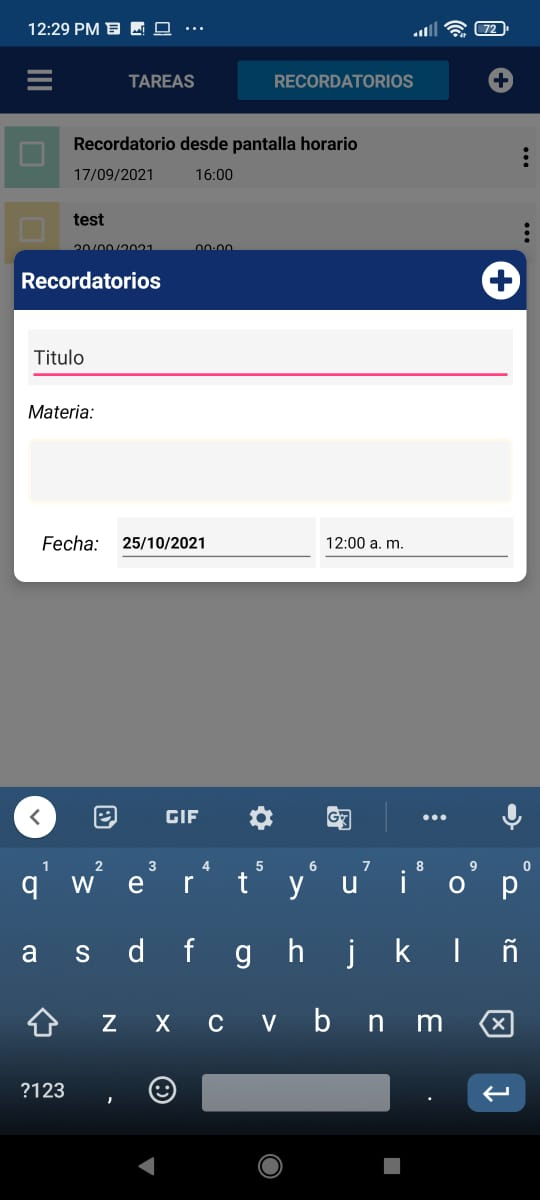
\includegraphics[width=.4\linewidth]{Imagenes/SOE10.jpeg} 
    \caption{En la opción recordatorio tenemos\\ cuatro campos para editar: Título, Materia,\\ Fecha de entrega,Hora de entrega} 
  \end{minipage}%% 
  \vspace{1cm}
  \begin{minipage}[b]{0.49\linewidth}
    \centering
    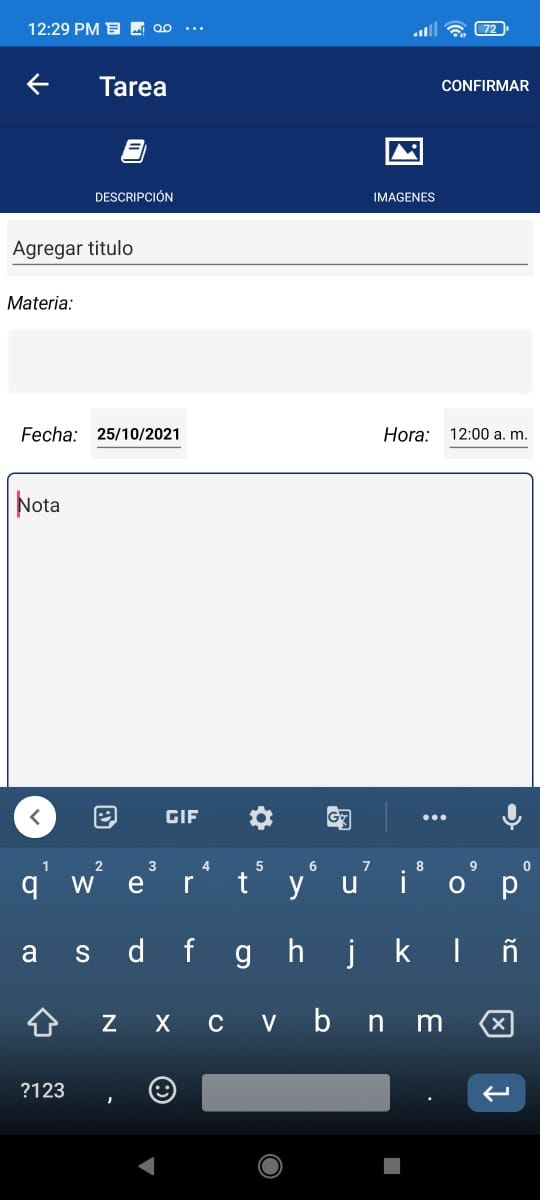
\includegraphics[width=.4\linewidth]{Imagenes/SOE11.jpeg} 
    \caption{En la opción tarea tenemos cuatro campos para editar: Título, Nota, Fecha de entrega, Hora de entrega, Imágenes} 
  \end{minipage} 
  \vspace{1cm}
\end{figure}

\newpage

\begin{figure}[ht!] 
  \begin{minipage}[b]{0.49\linewidth}
    \centering
    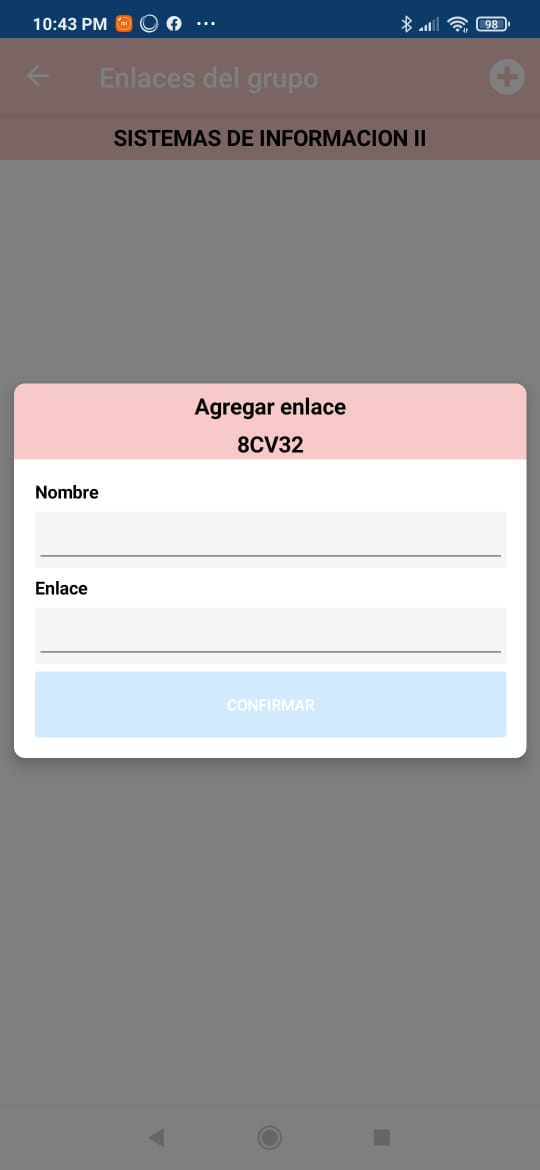
\includegraphics[width=.4\linewidth]{Imagenes/SOE13.jpeg} 
    \caption{Tenemos la opción de agregar un\\ enlace en la clase seleccionada como por\\ ejemplo una reunión en alguna plataforma.}
  \end{minipage}%%
  \vspace{1cm}
  \begin{minipage}[b]{0.49\linewidth}
    \centering
    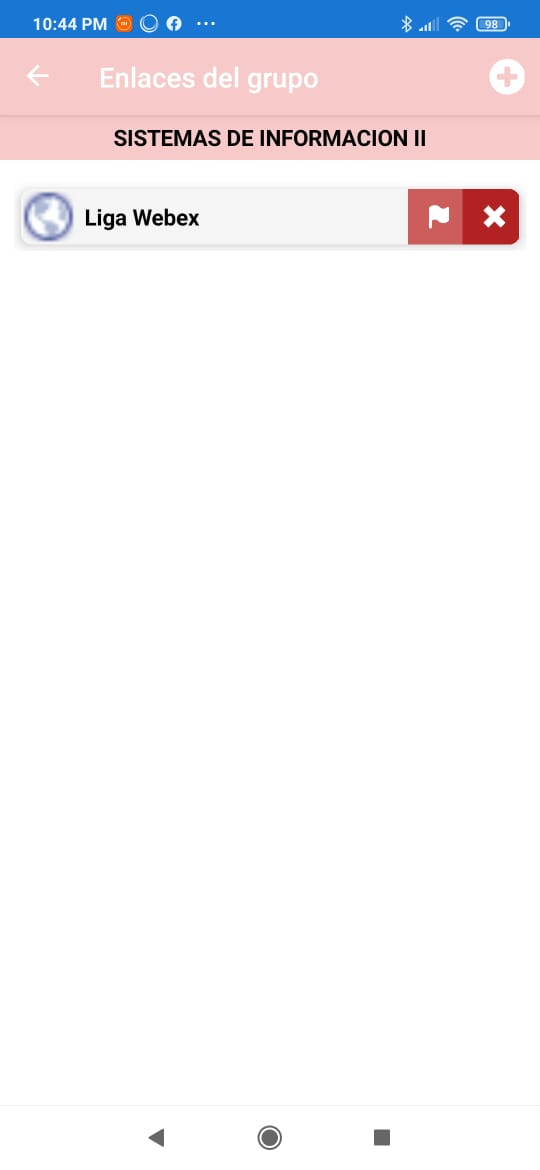
\includegraphics[width=.4\linewidth]{Imagenes/SOE14.jpeg} 
    \caption{Vista del enlace una vez creado, cualquier ususario puede ingresar a él presionando sobre el mismo.} 
  \end{minipage} 
  \vspace{1cm}
  \begin{minipage}[b]{0.49\linewidth}
    \centering
    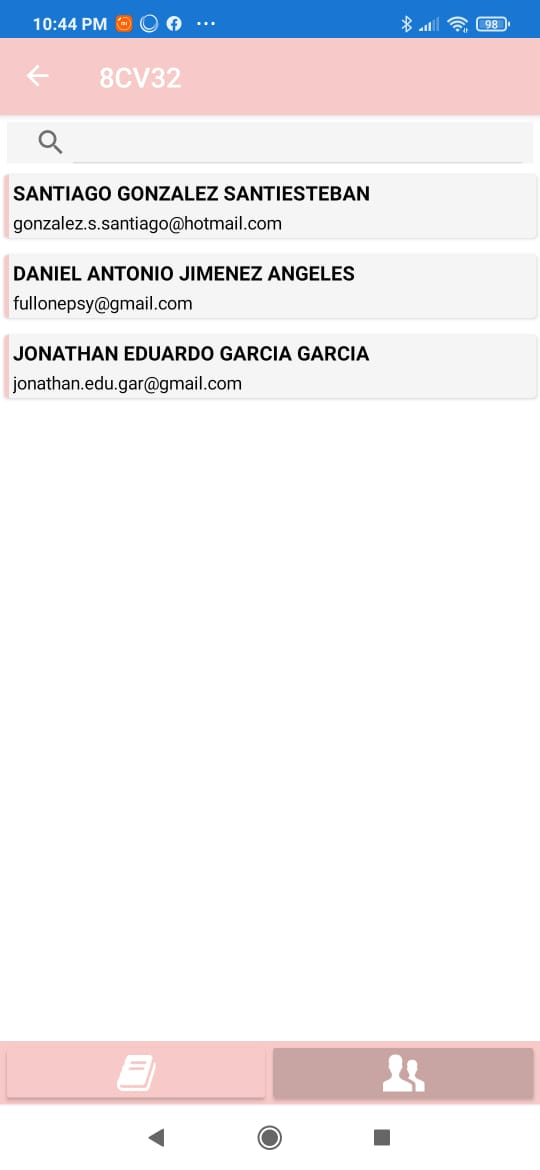
\includegraphics[width=.4\linewidth]{Imagenes/SOE15.jpeg} 
    \caption{Al seleccionar una materia podemos\\ ver a los alumnos pertenecientes al grupo.} 
  \end{minipage}%% 
  \vspace{1cm}
  \begin{minipage}[b]{0.49\linewidth}
    \centering
    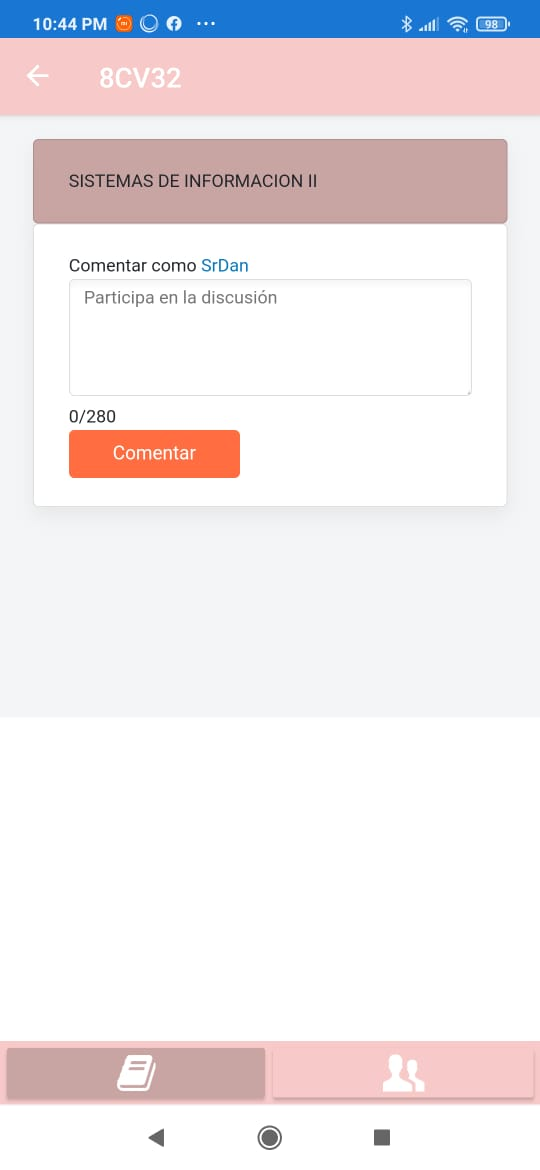
\includegraphics[width=.4\linewidth]{Imagenes/SOE16.jpeg} 
    \caption{La sección de comunidad permite a los alumnos pertenecientes a alguna de las clases publicar reseñas y comentarios que podrán visualizar otros alumnos pertenecientes al grupo.} 
  \end{minipage} 
  \vspace{1cm}
\end{figure}

\newpage

\section{Conclusión}
\justify
El presente proyecto de inicio a fin implicó retos importantes para cada uno de los miembros del equipo, de ellos podemos destacar el aprendizaje para obtener acceso en las implementaciones de las vistas de widget, notificaciones y otras funcionalidades nativas en cada plataforma así como en la homologación de la experiencia de usuario. Esta aplicación resuelve las necesidades que fueron identificadas durante la etapa de investigación del desarrollo. Durante la etapa de pruebas y puesta a disposición de los pilotos se observó una aceptación positiva por parte de los alumnos y su retroalimentación confirma que esta aplicación es de utilidad en la organización diaria de sus actividades escolares. Es importante destacar el apoyo que se tuvo por parte de las materias cursadas en la carrera que dieron las bases en el diseño y construcción de la aplicación.

%%%%%%% Bibliografía %%%%%%%%
\bibliographystyle{bst/IEEEtran.bst} 
\addcontentsline{toc}{section}{Referencias}  
\bibliography{bib/IEEEabrv,bib/IEEEreferencias.bib} 
%%%%%%% Bibliografía %%%%%%%%   

\section{Anexos}
\begin{itemize}
    \item \href{https://drive.google.com/file/d/15KZvm6CIDkM9g0DKMy8wb9b2fiIv2ROG/view?usp=sharing}
    {Diagrama arquitectura,  15 jun 2021}
    \item \href{https://drive.google.com/file/d/1LhLRHHiWVeEFRqgwnUttkpgct9kEACTq/view?usp=sharing} {Diseño Pantalla de tareas,  16 jun 2021}
    \item \href{https://drive.google.com/file/d/1N4PZQ41kn7JNZdWo4EaobB4sipUvPd8S/view?usp=sharing}{Recordatorios, 8 jul 2021}
    \item \href{https://drive.google.com/file/d/1NR3xwahN6aiRnEtGttwPc7ubX188eRmh/view?usp=sharing}{Modelo vista controlador,  6 abril 2021}
    \item \href{https://drive.google.com/file/d/1OMvjYk0Nwr1IXoy3Gtce-1zTW5y6Ea2j/view?usp=sharing}{Notas por materia, 11 jul 2021}
    \item \href{https://drive.google.com/file/d/1UC7XmlBGHwrKTog4K-RgmHMUh44nNHE9/view?usp=sharing}{Login, 25 jun 2021}
    \item \href{https://drive.google.com/file/d/1dKLuDtAksGwQyNf9vmHAt3SzZTOF-dzH/view?usp=sharing}{Pantalla información escolar, 17 ago 2021}
    \item \href{https://drive.google.com/file/d/1f6cP91edCqel2Af6U4ORgZ19fTHvJkgj/view?usp=sharing}{Esquema de notificaciones,  5 jul 2021}
    \item \href{https://drive.google.com/file/d/1gRQ1DOsUV1Sh1PLnGl-oD76absCRSu9o/view?usp=sharing}
{Esquema de servidor,  20 may}
    \item \href{https://drive.google.com/file/d/1iKIqTDIi4M3aPXLC7cX7fYwQdsycTmLQ/view?usp=sharing}
{Pantalla principal,  11 feb 2021}
    \item \href{https://drive.google.com/file/d/1tSR0xFik_Uz0kGiwxsTpW4rQPAiCZbmC/view?usp=sharing}
    {LinksPage,  1 ago 2021}
    \item \href{https://drive.google.com/file/d/1wgIdhQ5l7WvCdJyJS8HcCM8C_K1TBXVj/view?usp=sharing}{Archivero Virtual,  7 abr 2021}
    \item \href{https://drive.google.com/file/d/1ymBzTNposUKI1SH6fAeV3bMEkRAF2EMk/view?usp=sharing}{Tareas,  23 mar 2021}
    

\par\vspace{\baselineskip}

\end{itemize}

\end{document}